\documentclass[a4paper,onecolumn,oneside,12pt,extrafontsizes]{memoir}
\usepackage[utf8]{inputenc}
\usepackage[T1]{fontenc}
\usepackage[polish]{babel}
\usepackage{setspace}
\usepackage{tabularx}
\usepackage{color,calc}
\usepackage{ebgaramond}
\usepackage{tgtermes}   
\renewcommand*\ttdefault{txtt}
\usepackage{listings}
%%My Edits%%%%%%%%%%%%%%%%%
\usepackage{amsmath}
\usepackage{float}
\usepackage{amssymb}
\usepackage{minted}
\usepackage[ruled,vlined]{algorithm2e}\
\usepackage{afterpage}
%%%%%%%%%%%%%%%%%%%%%%%%%%%
\lstset{literate=%-
{ą}{{\k{a}}}1 {ć}{{\'c}}1 {ę}{{\k{e}}}1 {ł}{{\l{}}}1 {ń}{{\'n}}1 {ó}{{\'o}}1 {ś}{{\'s}}1 {ż}{{\.z}}1 {ź}{{\'z}}1 {Ą}{{\k{A}}}1 {Ć}{{\'C}}1 {Ę}{{\k{E}}}1 {Ł}{{\L{}}}1 {Ń}{{\'N}}1 {Ó}{{\'O}}1 {Ś}{{\'S}}1 {Ż}{{\.Z}}1 {Ź}{{\'Z}}1 
    {Ö}{{\"O}}1
    {Ä}{{\"A}}1
    {Ü}{{\"U}}1
    {ß}{{\ss}}1
    {ü}{{\"u}}1
    {ä}{{\"a}}1
    {ö}{{\"o}}1
    {~}{{\textasciitilde}}1
		{—}{{{\textemdash} }}1
}
\newcommand{\listingcaption}[1]
{
\vspace*{\abovecaptionskip}\small 
\refstepcounter{lstlisting}\hfill
Listing \thelstlisting: #1\hfill
\addcontentsline{lol}{lstlisting}{\protect\numberline{\thelstlisting}#1}
}
\lstset{
  breaklines=true,
  postbreak=\mbox{\textcolor{red}{$\hookrightarrow$}\space},
	belowskip=.5\baselineskip
}
\renewcommand\lstlistlistingname{Spis listingów}
\makeatletter
\g@addto@macro\insertchapterspace{\addtocontents{lol}{\protect\addvspace{10pt}}}
\renewcommand*{\l@lstlisting}{\@dottedtocline{1}{0em}{2.3em}}
\makeatother
\renewcommand*{\lstlistlistingname}{Spis listingów} \newlistof{lstlistoflistings}{lol}{\lstlistlistingname}
\clubpenalty=10000
\widowpenalty=10000
\righthyphenmin=3
\renewcommand{\topfraction}{0.95}
\renewcommand{\bottomfraction}{0.95}
\renewcommand{\textfraction}{0.05}
\renewcommand{\floatpagefraction}{0.35}
\setlength{\headsep}{10pt} 
\setlength{\headheight}{13.6pt}
\setlength{\footskip}{\headsep+\headheight}
\setlength{\uppermargin}{\headheight+\headsep+1cm}
\setlength{\textheight}{\paperheight-\uppermargin-\footskip-1.5cm}
\setlength{\textwidth}{\paperwidth-5cm}
\setlength{\spinemargin}{2.5cm}
\setlength{\foremargin}{2.5cm}
\setlength{\marginparsep}{2mm}
\setlength{\marginparwidth}{2.3mm}
\checkandfixthelayout[fixed]
\linespread{1}
\setlength{\parindent}{14.5pt}
\usepackage{memlays}
\usepackage{printlen}
\uselengthunit{pt}
\makeatletter
\newcommand{\showFontSize}{\f@size pt}
\makeatother
\usepackage{enumitem}
\setlist{noitemsep,topsep=4pt,parsep=0pt,partopsep=4pt,leftmargin=*}
\setenumerate{labelindent=0pt,itemindent=0pt,leftmargin=!,label=\arabic*.}
\setlistdepth{4}
\setlist[itemize,1]{label=$\bullet$}
\setlist[itemize,2]{label=\normalfont\bfseries\textendash}
\setlist[itemize,3]{label=$\ast$}
\setlist[itemize,4]{label=$\cdot$}
\renewlist{itemize}{itemize}{4}
\makeatletter
\renewenvironment{quote}{
	\begin{list}{}
	{
	\setlength{\leftmargin}{1em}
	\setlength{\topsep}{0pt}%
	\setlength{\partopsep}{0pt}%
	\setlength{\parskip}{0pt}%
	\setlength{\parsep}{0pt}%
	\setlength{\itemsep}{0pt}
	}
	}{
	\end{list}}
\makeatother
\DisemulatePackage{imakeidx}
\usepackage[makeindex,noautomatic]{imakeidx}
\makeindex
\makeatletter
\makeatother
\usepackage{ifpdf}
\ifpdf
 %MyEdit2 - \PassOptionsToPackage{hyphens}{url}
 \PassOptionsToPackage{hyphens}{url} \usepackage[pdftex,bookmarks,breaklinks,unicode]{hyperref}
 \usepackage[pdftex]{graphicx}
 \DeclareGraphicsExtensions{.pdf,.jpg,.mps,.png}
\pdfcompresslevel=9
\pdfoutput=1
\makeatletter
\AtBeginDocument{
  \hypersetup{
	pdfinfo={
    Title = {\@title},
    Author = {\@author},
    Subject={},
    Keywords={słowa kluczowe},  
		Producer={producer},
		Creator={pdftex}
	}}
}
\pdftrailerid{}
\pdfsuppressptexinfo15

\makeatother
\else
\usepackage{graphicx}
\DeclareGraphicsExtensions{.eps,.ps,.jpg,.mps,.png}
\fi
\sloppy
\setcounter{secnumdepth}{2}
\setcounter{tocdepth}{2}
\setsecnumdepth{subsection}
\makeatletter
\def\@seccntformat#1{\csname the#1\endcsname.\quad}
\def\numberline#1{\hb@xt@\@tempdima{#1\if&#1&\else.\fi\hfil}}
\makeatother
\renewcommand{\chapternumberline}[1]{#1.\quad}
\renewcommand{\cftchapterdotsep}{\cftdotsep}
\captionnamefont{\small}
\captiontitlefont{\small}
        \addto\captionspolish{
        \renewcommand{\tablename}{Tab.}
}


        \addto\captionspolish{
        \renewcommand{\figurename}{Rys.}
}


        \addto\captionspolish{
        \renewcommand{\bibname}{Bibliografia}
}

        \addto\captionspolish{
        \renewcommand{\listfigurename}{Spis rysunków} 
}

        \addto\captionspolish{
        \renewcommand{\listtablename}{Spis tabel}
}

        \addto\captionspolish{
\renewcommand\indexname{Indeks rzeczowy}
}
\addtopsmarks{headings}{
\nouppercaseheads
}{
\createmark{chapter}{both}{shownumber}{}{. \space}
\createmark{section}{right}{shownumber}{}{. \space}
}
\makeatletter
\copypagestyle{outer}{headings}
\makeoddhead{outer}{}{}{\small\itshape\rightmark}
\makeevenhead{outer}{\small\itshape\leftmark}{}{}
\makeoddfoot{outer}{\small\@author:~\@titleShort}{}{\small\thepage}
\makeevenfoot{outer}{\small\thepage}{}{\small\@author:~\@title}
\makeheadrule{outer}{\linewidth}{\normalrulethickness}
\makefootrule{outer}{\linewidth}{\normalrulethickness}{2pt}
\makeatother
\copypagestyle{plain}{headings}
\makeoddhead{plain}{}{}{}
\makeevenhead{plain}{}{}{}
\makeevenfoot{plain}{}{}{}
\makeoddfoot{plain}{}{}{}

\copypagestyle{empty}{headings}
\makeoddhead{empty}{}{}{}
\makeevenhead{empty}{}{}{}
\makeevenfoot{empty}{}{}{}
\makeoddfoot{empty}{}{}{}

\makeatletter
%Uczelnia
\newcommand\uczelnia[1]{\renewcommand\@uczelnia{#1}}
\newcommand\@uczelnia{}
%Wydział
\newcommand\wydzial[1]{\renewcommand\@wydzial{#1}}
\newcommand\@wydzial{}
%Kierunek
\newcommand\kierunek[1]{\renewcommand\@kierunek{#1}}
\newcommand\@kierunek{}
%Specjalność
\newcommand\specjalnosc[1]{\renewcommand\@specjalnosc{#1}}
\newcommand\@specjalnosc{}
%Tytuł po angielsku
\newcommand\titleEN[1]{\renewcommand\@titleEN{#1}}
\newcommand\@titleEN{}
%Tytuł krótki
\newcommand\titleShort[1]{\renewcommand\@titleShort{#1}}
\newcommand\@titleShort{}
%Promotor
\newcommand\promotor[1]{\renewcommand\@promotor{#1}}
\newcommand\@promotor{}
\def\maketitle{
  \pagestyle{empty}
	\fontfamily{\ebgaramond@family}\selectfont
	
\newlength{\tmpfboxrule}
\setlength{\tmpfboxrule}{\fboxrule}
\setlength{\fboxsep}{2mm}
\setlength{\fboxrule}{0mm} 
\setlength{\unitlength}{1mm}
\begin{picture}(0,0)
\put(26,-124){\fbox{
\parbox[c][71mm][c]{104mm}{\centering
\fontsize{16pt}{18pt}\selectfont \@title\\[5mm]
\fontsize{16pt}{18pt}\selectfont \@titleEN\\[20mm]
\fontsize{16pt}{18pt}\selectfont AUTOR:\\[2mm]
\fontsize{14pt}{16pt}\selectfont \@author}
}
}
\end{picture}
\setlength{\fboxrule}{\tmpfboxrule} 
	{\centering
		{\fontsize{22pt}{24pt}\selectfont \@uczelnia}\\[0.4cm]
		{\fontsize{22pt}{24pt}\selectfont \@wydzial}\\[0.5cm]
		  \hrule
	}
{\flushleft\fontsize{14pt}{16pt}\selectfont%
\begin{tabular}{ll}
KIERUNEK: & \@kierunek\\
SPECJALNOŚĆ: & \@specjalnosc\\
\end{tabular}\\[1.3cm]
}
{\centering
{\fontsize{32pt}{36pt}\selectfont PRACA DYPLOMOWA}\\[0.5cm]
{\fontsize{32pt}{36pt}\selectfont INŻYNIERSKA}\\[2.5cm]
}
\vfill
\begin{tabularx}{\linewidth}{p{6cm}X}
		&{\fontsize{16pt}{18pt}\selectfont PROWADZĄCY PRACĘ:}\\[2mm]
		&{\fontsize{14pt}{16pt}\selectfont \@promotor}\\[10mm]
		%&{\fontsize{16pt}{18pt}\selectfont OCENA PRACY:}\\[20mm]
	\end{tabularx}
\vspace{2cm}
\hrule\vspace*{0.3cm}
{\centering
{\fontsize{16pt}{18pt}\selectfont \@date}\\[0cm]
}
\normalfont
 \cleardoublepage
}
\makeatother

%%%%%%%%%%%%%%%%%%%%%%%%%%%%%%%%%%%%%%%%%
%%  Metadane dokumentu 
%%%%%%%%%%%%%%%%%%%%%%%%%%%%%%%%%%%%%%%%%
\title{Tworzenie mapy pomieszczenia za pomocą autonomicznej, mobilnej platformy skanującej}
\titleShort{Tworzenie mapy pomieszczenia za pomocą platformy skanującej}
\titleEN{Creating a room map using autonomous, mobile scanning platform}
\author{Tomasz Jakubowski}
\uczelnia{POLITECHNIKA WROCŁAWSKA}
\wydzial{WYDZIAŁ ELEKTRONIKI}
\kierunek{TELEINFORMATYKA}
\specjalnosc{PROJEKTOWANIE SIECI TELEINFORMATYCZNYCH}
\promotor{dr inż. Paweł Trajdos, K32W04D03}
\date{WROCŁAW, 2020}


\begin{document}
\newcommand\blankpage{%
    \null
    \thispagestyle{empty}%
    \addtocounter{page}{-1}%
    \newpage}
\afterpage{\blankpage}

\pdfbookmark[0]{Tytuł}{Tytul.1}
\maketitle


\chapterstyle{noNumbered}
\pagestyle{outer}
\mbox{}\pdfbookmark[0]{Spis treści}{spisTresci.1}
\tableofcontents* 

% \newpage
% \mbox{}\pdfbookmark[0]{Spis rysunków}{spisRysunkow.1}
% %\addcontentsline{toc}{chapter}{Spis rysunków}
% \listoffigures*

% \newpage
% \mbox{}\pdfbookmark[0]{Spis listingów}{spisListingow.1}
% %\addcontentsline{toc}{chapter}{Spis listingów}
% \lstlistoflistings*

% \newpage
% \mbox{}\pdfbookmark[0]{Spis tabel}{spisTabel.1}
% %\addcontentsline{toc}{chapter}{Spis tabel}
% \listoftables*

\chapter*{Słownik skrótów i pojęć}\mbox{}\pdfbookmark[0]{Słownik skrótów i pojęć}{skroty.1}
\label{sec:skroty}
\noindent
\begin{description}[labelwidth=*]
  \item  [IoT] (ang. \emph{Internet of Things}) \emph{Internet Rzeczy} - koncepcja przedmiotów codziennego użytku samodzielnie komunikujących się za pośrednictwem sieci Internet bądź innego środka w celu gromadzenia i przetwarzania danych
  
  \item [ToF] (ang. \emph{Time of Flight}) \emph{Czas lotu} - tutaj w odniesieniu do rodzaju sensora laserowego mierzącego dystans za pomocą pomiaru czasu jaki upływa od wysłania impulsu świetlnego do odebrania jego odbicia od przeszkody
  
  \item [SLAM] (ang. \emph{Simultaneous Localization And Mapping}) \emph{Symultaniczna lokalizacja i mapowanie} - problem obliczeniowy dotyczący jednoczesnego tworzenia obrysu obiektów w otoczeniu na podstawie pomiarów i znanej lokalizacji jednostki mierzącej w przestrzeni oraz określenia położenia jednostki mierzącej w otoczeniu na podstawie dokonywanych przez nią pomiarów
  
  \item [VSLAM]
  
  \item [LIDAR]
  
  \item [PC] (ang. \emph{Personal Computer}) \emph{Komputer Osobisty}
  
  \item [smart] (z ang. \emph{sprytny})  - w kontekście tego dokumentu jest to jedno z haseł często występujących w nazwach i reklamach produktów wyposażonych w dowolnego rodzaju mikrokomputer z oprogramowaniem pozwalającym na komunikację sprzętu z aplikacją na smartfona bądź interfejsem przeglądarkowym, rzekomo ułatwiającym korzystanie z niego. Ubarwia ono obraz urządzenia w oczach konsumenta mając przekonać go do jego innowacyjności. 
  
  \item [intelligent] (z ang. \emph{inteligentny})  - podobnie jak ``smart`` w kontekście niniejszej pracy jest często wykorzystywanym określeniem nowoczesnych produktów
  
  \item [Firmware] - oprogramowanie wbudowane działające na mikrokontrolerze
  
  \item [Arduino] - rodzaj płytek drukowanych z wbudowanymi mikrokontrolerami o publicznie dostępnych schematach elektronicznych, również otwartoźródłowe środowisko służące do pisania, kompilacji i wgrywania programów na płytki
  
  \item [STM32duino] - nieoficjalna implementacja środowiska kompilacji (bibliotek) Arduino dla płytek z mikrokontrolerami STM32
  
\end{description}

\chapterstyle{default}
\chapter{Wstęp}
\section{Wprowadzenie}
Niniejszy \cite{Kedzierski2016} dokument\cite{GettingStartedWithProcessing} powstał \cite{Borenstein1995} z myślą o ujednoliceniu sposobu redagowania prac dyplomowych. Jego źródła mają pełnić rolę szablonu nowoedytowanej pracy, zaś treść powinna być interpretowana jako zestaw zaleceń i uwag o charakterze technicznym (dotyczących takich zagadnień, jak: formatowanie tekstu, załączanie rysunków, układ strony itp.) oraz stylistycznym (odnoszących się do stylu wypowiedzi, sposobów tworzenia referencji itp.).

Szablon przygotowano do kompilacji pdflatexem w konfiguracji: \texttt{MiKTeX} (windowsowa dystrybucja latexa) + \texttt{TeXnicCenter} (środowisko do edycji i kompilacji projektów latexowych) + \texttt{SumatraPDF} (przeglądarka pdfów z nawigacją zwrotną) + JabRef (opcjonalny edytor bazy danych bibliograficznych). Jest to zalecany zestaw narzędzi do edycji pracy w systemie Windows. Można je pobrać ze stron internetowych, których adresy zamieszczono w tabeli~\ref{tab:narzedzia}.
\begin{table}[htb] \small
\centering
\caption{Wykaz zalecanych narzędzi do kompilacji szablonu (adresy internetowe ważne na dzień 1.04.2016)}
\label{tab:narzedzia}
\begin{tabularx}{\linewidth}{|c|c|X|p{6cm}|} \hline\
Narzędzie & Wersja & Opis & Adres \\ \hline\hline
MiKTeX & 2.9 & Zalecana jest instalacja \texttt{Basic MiKTeX} z dystrubucji 32 lub 64 bitowej. Brakujące pakiety będą się doinstalowywać podczas kompilacji projektu. &
\url{http://miktex.org/download} \\ \hline
TexnicCenter & 2.02 &  Można pobrać 32 lub 64 bitową wersję & \url{http://www.texniccenter.org/download/} \\ \hline
SumatraPDF & 3.1.1 & Można pobrać 32 lub 64 bitową wersję & \url{http://www.sumatrapdfreader.org/download-free-pdf-viewer.html} \\ \hline
JabRef & 3.3 & Można pobrać 32 lub 64 bitową wersję & \url{http://www.fosshub.com/JabRef.html} \\ \hline
\end{tabularx}
\end{table}
Nic nie stoi jednak na przeszkodzie, aby szablon ten dostosować do wykorzystania z użyciem innych narzędzi. Dostosowanie to mogłoby polegać na zmianie kodowania plików i korekcie deklaracji kodowania znaków w dokumencie głównym (co opisano dalej).

W kodzie źródłowym szablonu zamieszczono komentarze z uwagami pozwalającymi lepiej zrozumieć znaczenie używanych komend. Komentarze te nie są widoczne w pliku \texttt{Dokument.pdf}, który powstaje jako wynik kompilacji szablonu. 


%%%2. środowisko do pisania kodu latexa: 
%%%( )
%%%3. viewer pdf-ów, pozwalający na nawigację zwrotną: Sumatra PDF 3.0
%%%(http://www.sumatrapdfreader.org/download-free-pdf-viewer.html)
%%%
%%%- o konfiguracji texniccenter do współdziałania z sumatra pdf można poczytać sobie na stronie:
%%%http://tex.stackexchange.com/questions/116981/how-to-configure-texniccenter-2-0-with-sumatra-2013-2014-2015-version
%%%(można znaleźć też inne tutoriale)
%%%
%%%4. środowisko do zarządzania bibliografią: JabRef
%%%(http://jabref.sourceforge.net/download.php)
%%%
%%%Polecam też instalację pod windowsami następujących narzędzi:
%%%- Sumatra PDF - przeglądarka pdf umożliwiająca nawigację pomiędzy
%%%edytowanym tekstem a przeglądanym dokumentem (podglądanie tekstu w
%%%TeXnicCenter umieszcza kursor w odpowiednim miejscu w pdfie, podwójne
%%%kliknięcie w pdfie ustawia kursor w edytorze tekstu).
%%%- JabRef - narzędzie do przygotowywania bibliografii.
%%%
%%%
%%%Uwaga: tytuł powinien zmieścić się w okienku kolorowej okładki (którą
%%%powinna dostarczyć uczelniana administracja). Proszę posterować
%%%parametrami, aby "wpasować" w okienko własny tekst.
%%%
%%%Do ASAPa należy wprowadzić pracę dyplomową/projekt inżynierski w pliku o nazwie:
%%%
%%%W04_[nr albumu]_[rok kalendarzowy]_[rodzaj pracy] (szczegółowa instrukcja pod adresem asap.pwr.edu.pl)
%%%
           %%%Przykładowo:
        %%%­W04_123456_2015_praca inżynierska.pdf     - praca dyplomowa inżynierska
        %%%W04_123456_2015_projekt inżynierski.pdf   - projekt inżynierski
        %%%W04_123456_2015_praca magisterska.pdf  - praca dyplomowa magisterska
%%%
              %%%rok kalendarzowy ? rok realizacji kursu „Praca dyplomowa” (nie rok obrony) 
\chapter{Projekt}
\section{Oprogramowanie PC}
\subsection{Struktura oprogramowania}
Robot wykonuje polecenia zadane przez aplikację sterującą oraz odpowiada na zapytania o dane. Aplikacja w ostatecznej wersji została zaimplementowana jako moduł platformy ROS\cite{ros} na systemie operacyjnym opartym o GNU/Linux. Po jej uruchomieniu ukazują się dwa okna - jedno jest oknem głównym do kontroli pojazdu, widoczne na Rys. \ref{fig:app-main-window}. Drugie to okno programu RViz w którym widoczny jest podgląd pozycji robota oraz mapy którą sporządza ukazane na Rys. \ref{fig:rviz-window}.

\subsubsection{Okno główne programu}
\begin{figure}[ht]
	\centering
		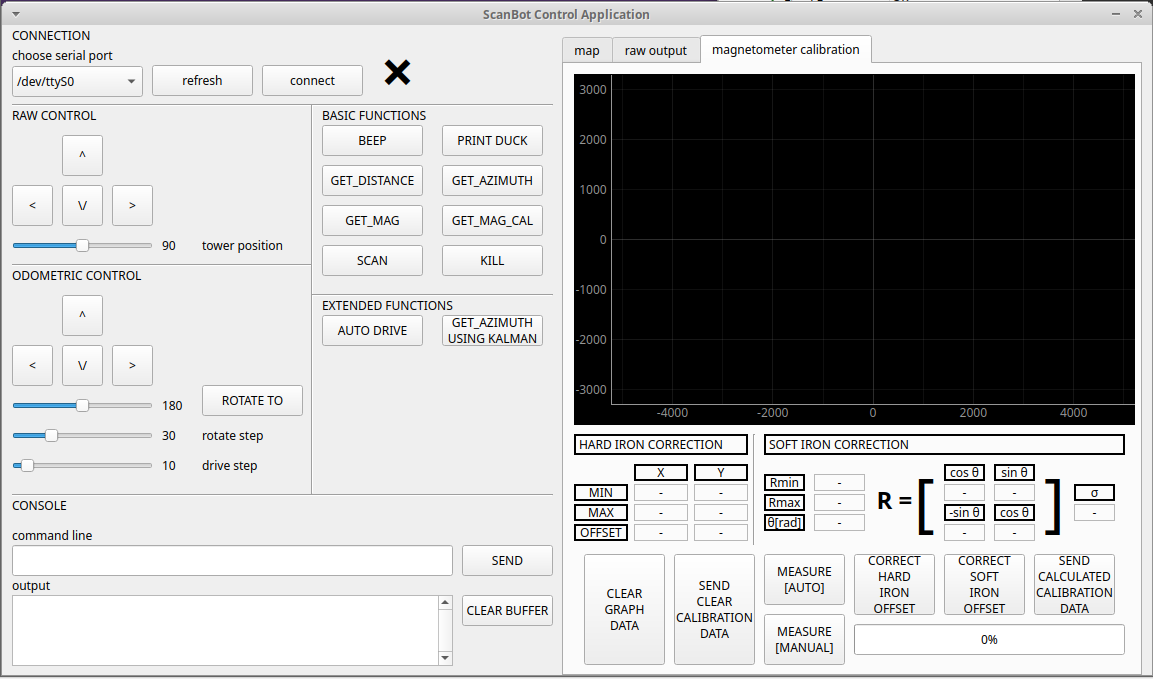
\includegraphics[width=1\linewidth]{rys/main-app-view-3.PNG}
	\caption{Okno główne aplikacji sterującej}
	\label{fig:app-main-window}
\end{figure}

Okno główne zostało podzielone na segmenty oraz zakładki w celu odseparowania poszczególnych funkcjonalności. Opis poszczególnych sekcji:

Sekcja \emph{CONNECTION} dotyczy połączenia portu szeregowego i zawiera elementy takie jak:
\begin{itemize}
    \item Lista rozwijana do wyboru portu szeregowego do którego wpięty jest konwerter USB-UART
    \item Przycisk \emph{refresh} odświeża listę
    \item Przycisk \emph{connect} inicjuje połączenie
    \item Ikona statusu połączenia - krzyżyk oznacza jego brak, zegarek oznacza oczekiwanie a symbol fajki oznacza zainicjowane połączenie
\end{itemize}

Sekcja \emph{RAW CONTROL} zawiera kontrolki sterujące robotem. Przytrzymanie każdego z przycisków odpowiada ruchowi robota w przód i w tył (kolejno strzałki w górę i w dół) lub obrotowi w lewo i w prawo (strzałki w lewo i w prawo). Po puszczeniu przycisku platforma zatrzymuje się bez zwłoki. Suwak służy do ustawiania pozycji wieżyczki pomiarowej, jest wyskalowany w stopniach.
\\

Sekcja \emph{ODOMETRIC CONTROL} służy do jazdy odometrycznej, tj. poruszając się za pomocą tych kontrolek uwzględniany jest przejechana trasa. Analogicznie jak w poprzedniej sekcji poruszanie kontrolowane jest przez strzałki, aczkolwiek tutaj nie należy ich przytrzymywać a jedynie krótko kliknąć. Po kliknięciu zostanie pokonany pewien dystans po którym robot się zatrzyma. Dystans do przejechania (krok) ustawiany jest za pomocą suwaka \emph{drive step} a wartość przez niego reprezentowana jest podana w centymetrach. Aby ustawić krok obrotu należy skorzystać z suwaka \emph{rotate step}. Przycisk \emph{ROTATE TO} służy do obracania robota na wyznaczony azymut, którego wartość wcześniej należy ustawić suwakiem znajdującym się obok niego. (Uwaga! Pojęcie azymutu w tym dokumencie jest użyte w odniesieniu do zmiennej trzymającej aktualny kąt skierowania robota, nie azymtu geograficznego. Więcej o tym znajduję się w rozdziale [>TODO dac ref do miejsca gdzie to będzie obszernie wytłumaczone].
\\

Sekcja \emph{CONSOLE} pozwala na ręczne sterowanie robotem za pośrednictwem komend. Tutaj należy zaznaczyć że wszysktie funkcje sterujące oferowane przez program korzystają z tych komend odpowiednio je formułując i wysyłając do jednostki mobilnej. Pole tekstowe podpisane \emph{command line} służy do wprowadzania komendy, która jest wysyłana po kliknięciu przycisku \emph{SEND}.
Owa komenda pojawi się wtedy w polu tekstowym poniżej oznaczonym \emph{output}. Przycisk \emph{CLEAR BUFFER} wyczyści okno podglądu wraz z buforem nadawczym i odbiorczym, co przydaje się przy (na szczęście bardzo rzadkich) problemach z zerwaną komunikacją lub utratą synchronizacji sekwencji przesyłanych komend i odpowiedzi.
\\

Sekcja \emph{BASIC FUNCTIONS} posiada kolekcję przycisków wykonujących podstawowe funkcje robota niezwiązane z poruszaniem.
\begin{itemize}
    \item \emph{BEEP} powoduje wydanie 3 krótkich dźwięków przez robota
    \item \emph{PRINT DUCK} rysuje małą kaczkę na ekranie
    \item \emph{GET\_DISTANCE} mierzy i zwraca odległość od robota do przeszkody na którą aktualnie wycelowana jest wieżyczka
    \item \emph{GET\_AZIMUTH} mierzy i zwraca azymut w którym skierowany jest robot
    \item \emph{GET\_MAG} zwraca surowe dane z magnetometru (osie X i Y)
    \item \emph{GET\_MAG\_CAL} zwraca dane kalibracji magnetometru
    \item \emph{SCAN} skanuje otoczenie (obraca wieżyczkę i dokonuje serii 180 pomiarów odległości), po czym zwraca zmierzone wartości
    \item \emph{KILL} odłącza sygnał sterujący od serwomechanizmów
\end{itemize}

Sekcja \emph{EXTENDED FUNCTIONS} pozwala na wykonywanie bardziej złożonych zadań
\begin{itemize}
    \item \emph{AUTO DRIVE} załącza algorytm autonomiczej jazdy robota
    \item \emph{GET\_AZIMUTH USING KALMAN} wykonuje serię pomiarów i za pomocą prostej implementacji filtru Kalmana\cite{Kedzierski2016} zwraca przefiltrowany wynik reprezentujący azymut w którym robot jest skierowany
\end{itemize}

Zakładka \emph{map} zawiera wykres który służy do wyświetlania zmierzonych punktów na układzie współrzędnych

Zakładka \emph{raw output} zawiera pełnowymiarowy podgląd na historię wysyłanych i odbieranych danych. Jest większą wersją okienka \emph{output} sekcji \emph{CONSOLE}

Zakładka \emph{magnetometer calibration} zawiera zestaw elementów wykorzystywanych do kalibracji magnetometru. Więcej o tej zakładce jak i o przebiegu kalibracji w podrozdziale \ref{sec:mag_cal}.

\subsubsection{Program RViz}
\begin{figure}[ht]
	\centering
		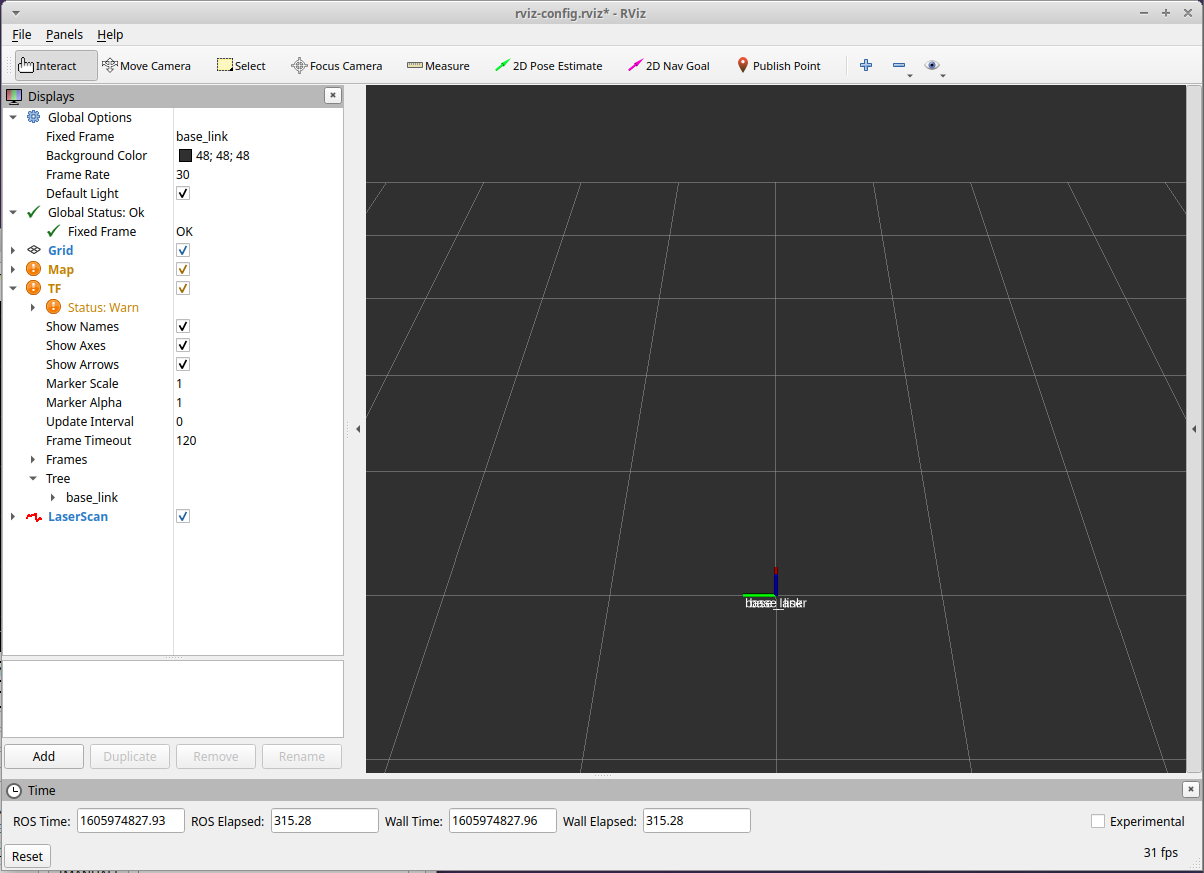
\includegraphics[width=1\linewidth]{rys/main-app-view-4.PNG}
	\caption{Okno programu RViz}
	\label{fig:rviz-window}
\end{figure}

Z okna głównego programu RViz należy zwrócić uwagę jedynie na podgląd układu współrzędnych po prawej stronie okna. Wszystkie parametry są ustawiane automatycznie wraz ze startem aplikacji, nie ma potrzeby żadnej ręcznej konfiguracji. Więcej informacji o tym programie dostępne jest na stronie internetowej \cite{rviz}.
Podczas pracy programu aktualna pozycja robota jest reprezentowana jako obiekt z etykietą \emph{base\_link} - podczas jazdy jego pozycja jest aktualizowana względem etykiety \emph{odom}. Na początku wszystkie układy współrzędnych są w pozycji zerowej i się nakładają.

\subsubsection{Środowisko sterujące}
\label{sec:ros-env}
\begin{figure}[ht]
	\centering
		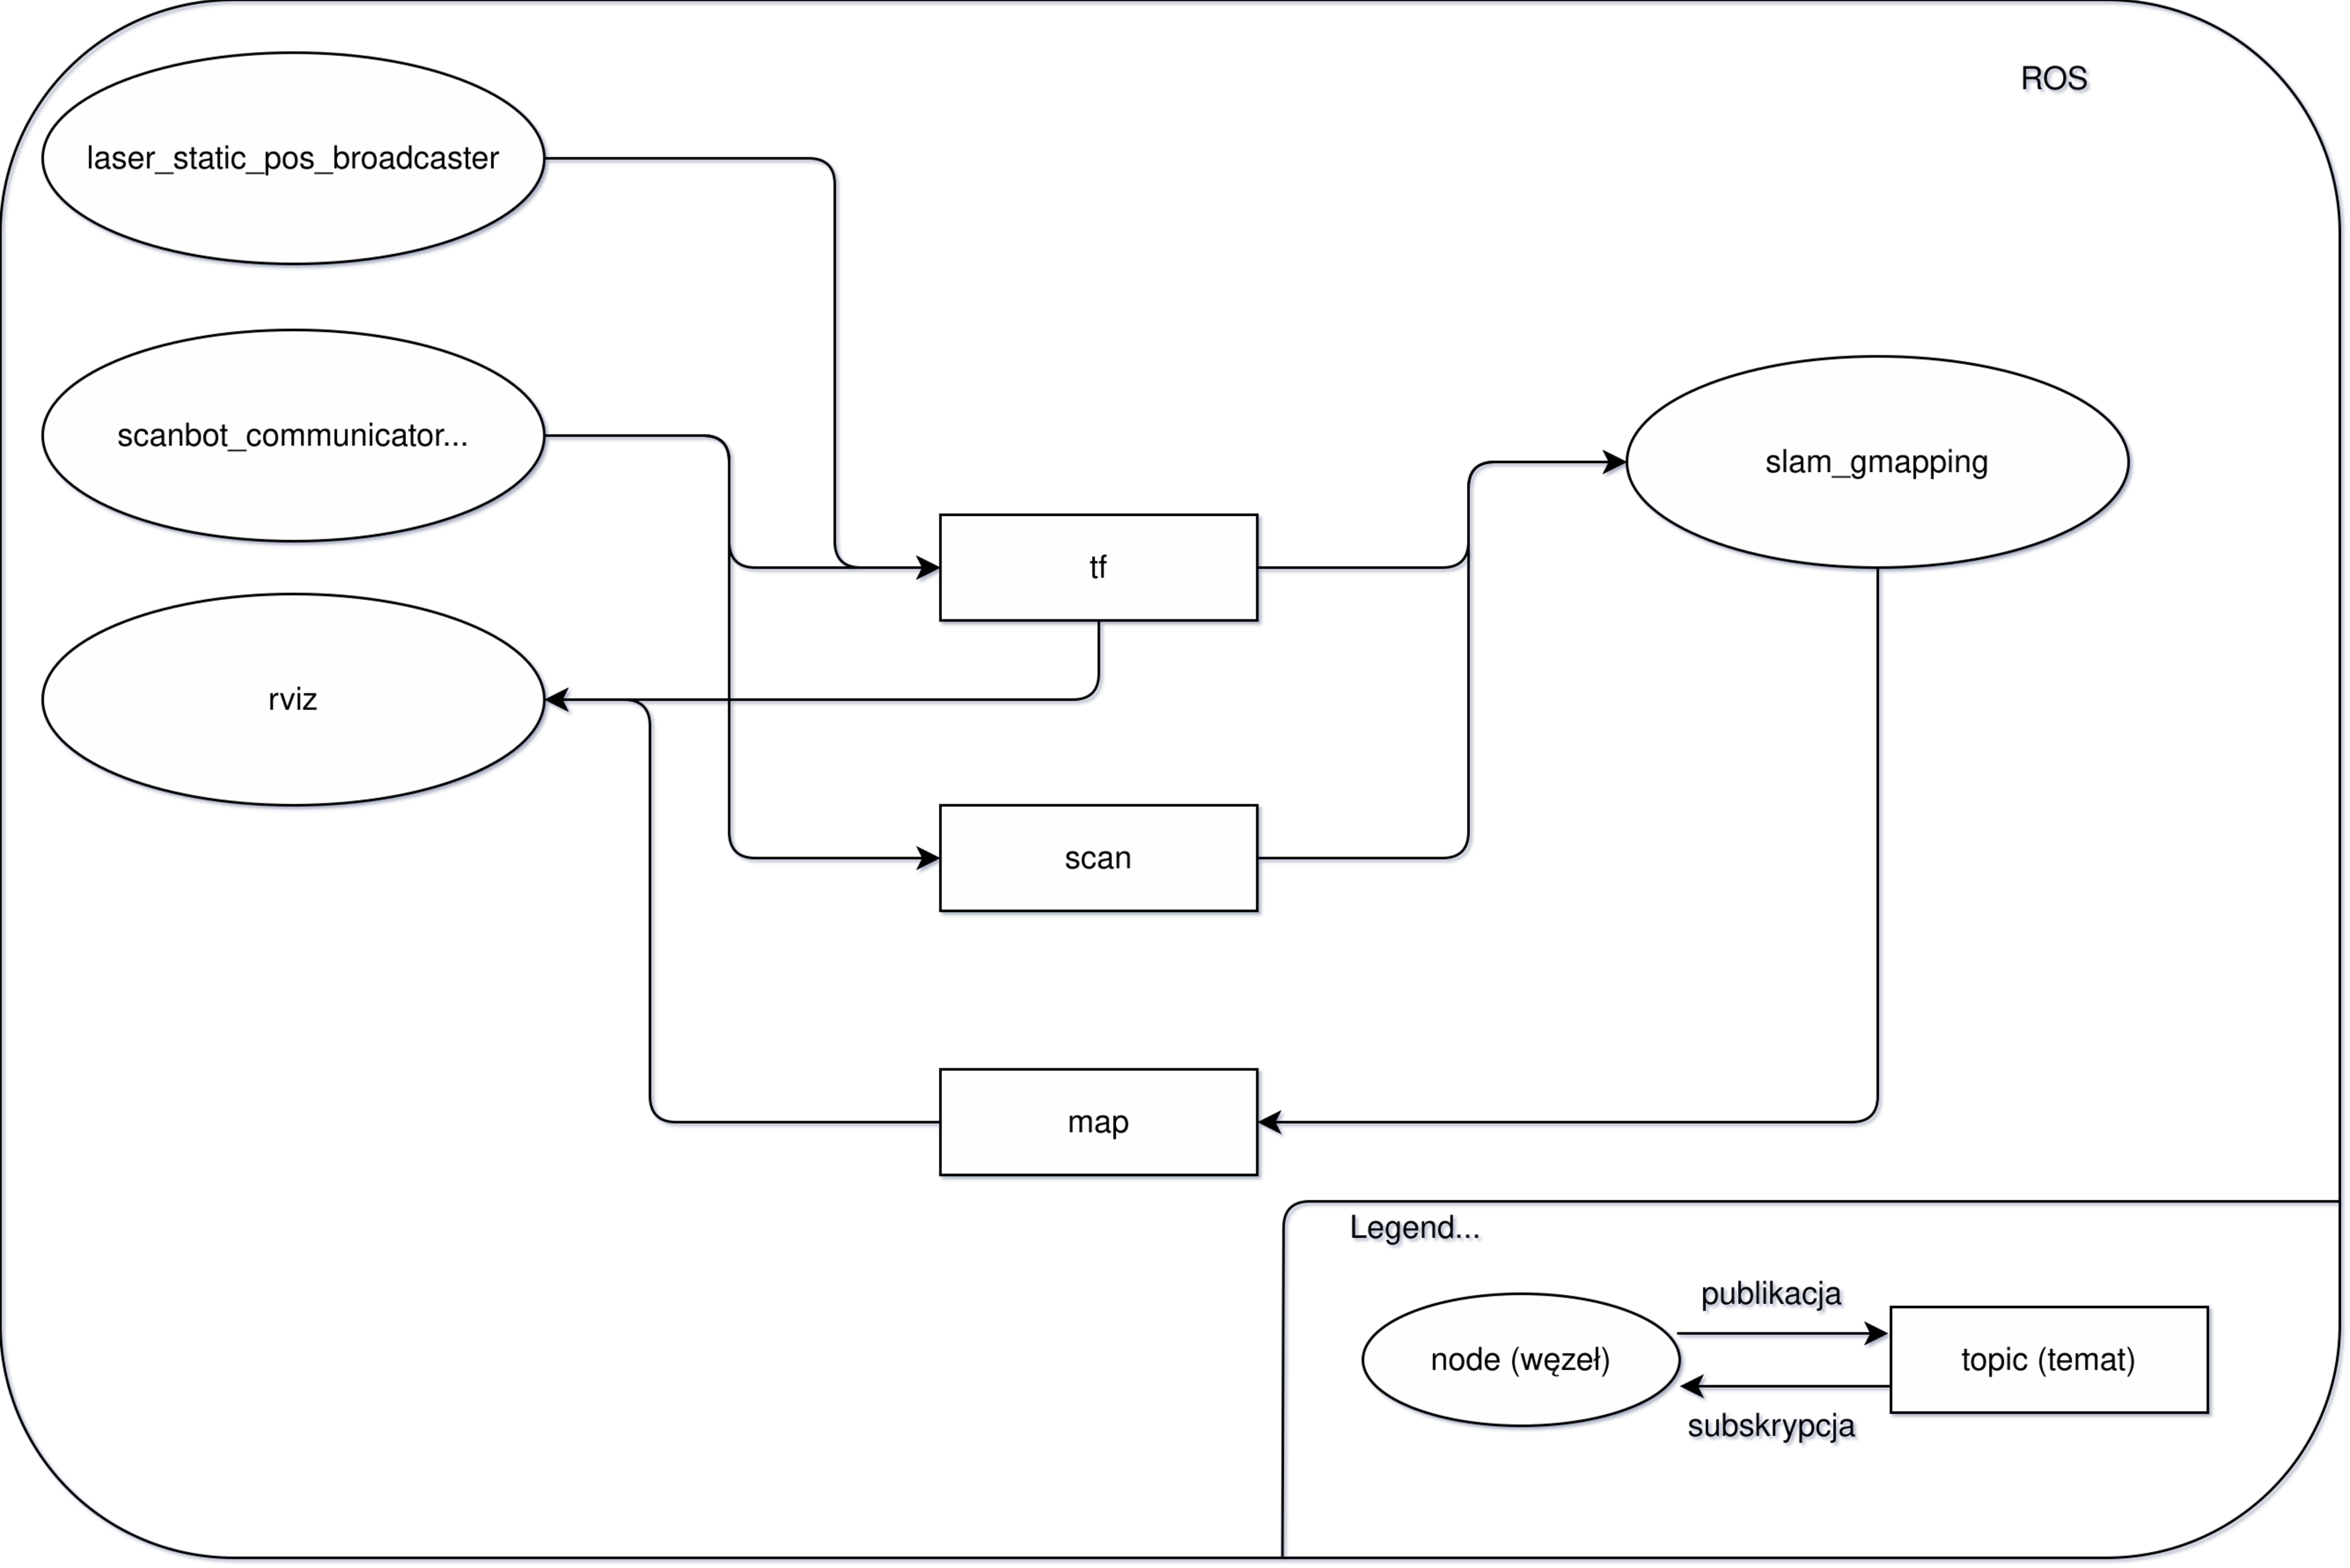
\includegraphics[width=1\linewidth]{rys/pc-application-infrastructure.pdf}
	\caption{Struktura środowiska ROS}
	\label{fig:pc-app-ros-infrastructure}
\end{figure}

Aplikacja komputerowa po uruchomieniu w środowisku ROS widoczna jest jako jeden z węzłów (node). W celu sporządzania mapy komunikuje się z innymi węzłami za pośrednictwem tematów (topics).
Na Rys. \ref{fig:pc-app-ros-infrastructure} ukazany jest schemat komunikacji poszczególnych węzłów.
Wykorzystywane są trzy tematy:
\begin{itemize}
    \item \emph{tf} jest tematem na którym publikowane są wszelkie translacje, czyli zależności między układami odniesienia
    \item \emph{scan} - tutaj publikowane są wyniki pomiarów odległości po wykonaniu skanu przez robota
    \item \emph{map} - na tym temacie pojawiają się dane reprezentujące mapę, wygenerowane przez algorytm \emph{gmapping}\cite{Grisetti2005}\cite{gmapping-website}\cite{gmapping-ros}
\end{itemize}

Ramki (frames), czyli w terminologii stosowanej w ROS układy odniesienia, a konkretnie ich względna pozycja są reprezentowane za pomocą wektorów zawierających dane o przesunięciu jak i obrocie. Więcej informacji na temat szczegółowego działania ramek można zasięgnąć na stronie internetowej ROS'a\cite{ros}. W niniejszym projekcie wykorzystywane są 4 ramki:
\begin{itemize}
    \item \emph{map} to główny układ odniesienia względem którego rysowana jest mapa
    \item \emph{odom} jest punktem odniesienia względem którego działa algorytm nawigacji zliczeniowej
    \item \emph{base\_link} odnosi się do bazy pojazdu, tj. środka względem którego się obraca podczas zakręcania
    \item \emph{base\_laser} to pozycja sensora skanującego
\end{itemize}
Wsyzstkie translacje między ramkami publikowane są na temacie \emph{tf}.

Węzeł \emph{laser\_static\_pod\_broadcaster} cyklicznie publikuje informację o położeniu modułu skanującego względem bazy robota. Jako że znajduje się ona bezpośrednio nad środkiem obrotu platformy, a sporządzana mapa jest dwuwymiarowa, jest to wektor zerowy.

Węzeł \emph{scanbot\_communicator} publikuje swoją pozycję na temacie \emph{tf} oraz podczas wykonywania skanu na kanale \emph{scan}.

Węzeł \emph{slam\_gmapping} subskrybuje kanały \emph{tf} i \emph{scan}. Na ich podstawie odpowiednio filtrując punkty uzyskane z pomiarów i dopasowując je do poprzednich algorytm tworzy mapę przeszkód widzianych przez robota.

Węzeł \emph{rviz} reprezentuje program RViz i subskrybuje dwa tematy - \emph{tf} oraz \emph{map}. Pozycje układów odniesienia reprezentowane są prze trójkolorowe trójwymiarowe obiekty, gdzie każdy z kolorów odpowiada jednej z osi (czerwony, zielony, niebieski odpowiadają kolejno osiom X, Y oraz Z). Ich położenie jest znane dzięki subskrypcji pierwszego z wymienionych tematów. Za pomocą danych przychodzących z drugiego z nich, program rysuje mapę pomieszczenia.


\subsubsection{Struktura aplikacji sterującej}
\begin{figure}[ht]
	\centering
		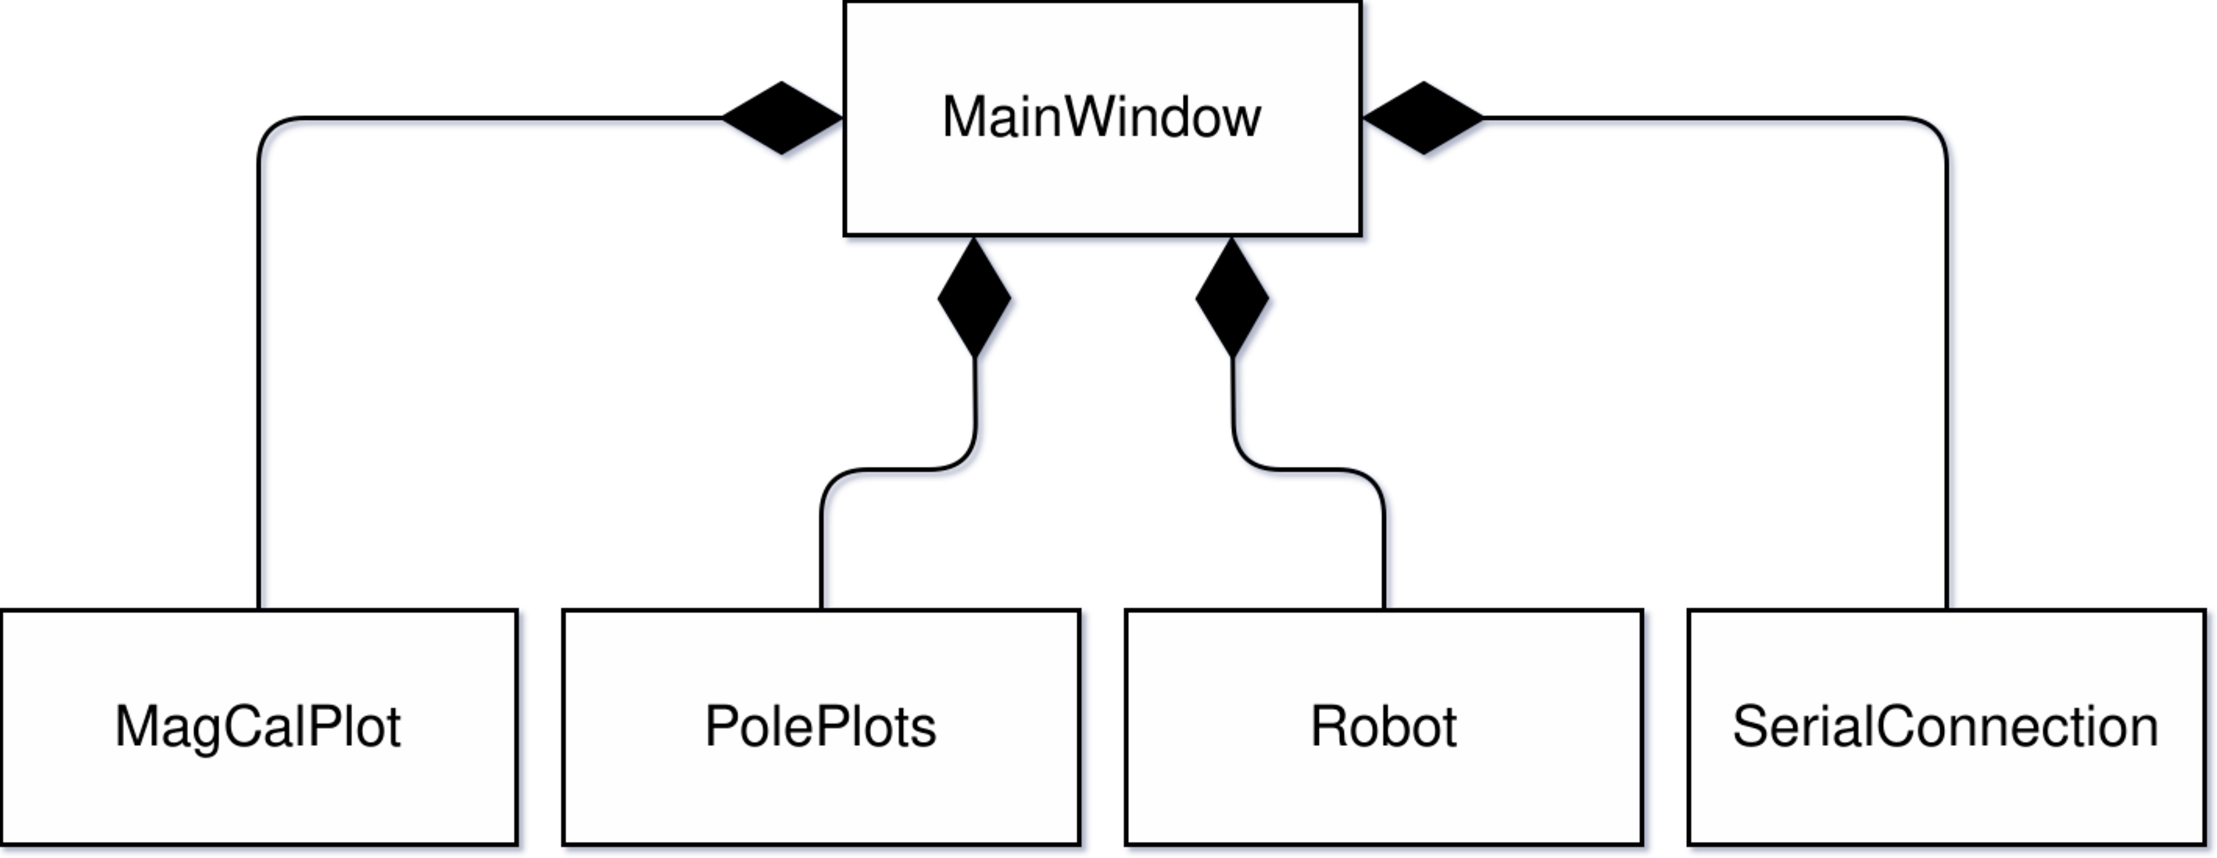
\includegraphics[width=0.8\linewidth]{rys/pc-application-simplified-uml.pdf}
	\caption{Uproszczony diagram kluczowych klas aplikacji}
	\label{fig:simple-class-diagram}
\end{figure}

W tej sekcji przedstawiony zostanie zarys najbardziej znaczących klas aplikacji sterującej. Jako że sama jej budowa nie jest kluczowym aspektem niniejszej pracy, dlatego po szczegółowe informacje dotyczące jej funkcjonowania autor odsyła do kodu źródłowego znajdującego się w dodatku A.

Na diagramie \ref{fig:simple-class-diagram} ukazano najważniejsze klasy głównego programu. Głównym obiektem jest tutaj okno, instancja klasy \emph{MainWindow}. Tutaj obsłużone jest kreowanie interfejsu graficznego, czyli ustawienie przycisków, pól tekstowych i innych elementów w odpowiednich miejscach, nadanie im identyfikatorów, ustawienie ciągów tekstowych, suwaków i innych elementów graficznych. Również akcje towarzyszące kliknięciom przycisków i przesuwaniu suwaków są tutaj przypisywane do odpowiednich funkcji. Funkcje te dla lepszej organizacji oraz czytelności zostały przeniesione do innych klas zorientowanych wokół konkretnych segmentów pracy aplikacji. Obiekty tych klas dostępne są poprzez zmienne wewnątrz głównej klasy.
\\

Klasa \emph{MagCalPlot} obsługuje szereg funkcji związanych z kalibracją magnetometru \ref{sec:mag_cal}. Zawiera przyciski uruchamiające funkcje związane z:
\begin{itemize}
    \item Czyszczeniem wykresu
    \item Rysowaniem zmierzonych danych w postaci punktów na wykresie
    \item Automatycznym pomiarem surowych danych z magnetometru
    \item Ręcznym pomiarem surowych danych z magnetometru
    \item Korekcją błędu \emph{hard iron} \cite{hard-iron} \cite{hard-soft-iron}
    \item Korekcją błędu \emph{soft iron} \cite{hard-soft-iron}
    \item Wysyłaniem danych kalibracyjnych do robota
\end{itemize}

Klasa \emph{PolePlots} obsługuje rysowanie punktów oraz czyszczenie wykresu zakładki \emph{map}. Przechowuje również dane o kolorach punktów jakie są na nim rysowane.

Klasa \emph{Robot} odzwierciedla surowy interfejs robota \label{sec:firmware}, dodając warstwę abstrakcji na surowe komendy wydawane mobilnej platformie i rozszerzając je - przykładowo podczas każdego z wywołanych funkcją pomiarów azymutu, jest on od razu publikowany na temacie \emph{tf}. Dodatkowo, w tej klasie obsłużony jest pomiar azymutu za pośrednictwem filtru Kalmana \cite{Kedzierski2016}. Również tutaj obsłużone jest publikowanie danych z odometrii i wykonywanych skanów na odpowiednich tematach, opisanych wcześniej w sekcji \ref{sec:ros-env} jak i również algorytm samodzielnej jazdy robota.

Klasa \emph{SerialConnection} służy do obsługi komunikacji interfejsu szeregowego konwertera USB-UART. Zawiera funkcje służące do nawiązywania połączenia, wysyłania komend i odbierania odpowiedzi od robota. Ponadto posiada uchwyt do klasy głównej, dzięki czemu wymieniane dane prezentuje zarówno w polu tekstowym w sekcji okna \emph{CONSOLE} jak i w zakładce \emph{raw output}.

\subsection{Jazda autonomiczna}
W celu realizacji samodzielnej jazdy robot został wyposażony w autorski algorytm pozwalający na omijanie napotkanych przeszkód i poruszanie się wzdłuż ścian. Operuje on na bardzo prostych zasadach - robot wykonuje kroki, pomiędzy którymi skanuje otoczenie i decyduje o podjętej akcji. Decyzja zapada na podstawie wykrycia przeszkód w wyznaczonych strefach. Ze względu na powiązanie z napisanym programem Rys. \ref{fig:autodrive-zones} przedstawia angielskie nazwy tychże stref. Ich kształt został wybrany ze względu na prostotę implementacji.
\begin{itemize}
    \item \emph{FRONT ZONE} (strefa F)
    \item \emph{LEFT ZONE 1} (strefa L1)
    \item \emph{LEFT ZONE 2} (strefa L2)
\end{itemize}

\begin{figure}[ht]
	\centering
		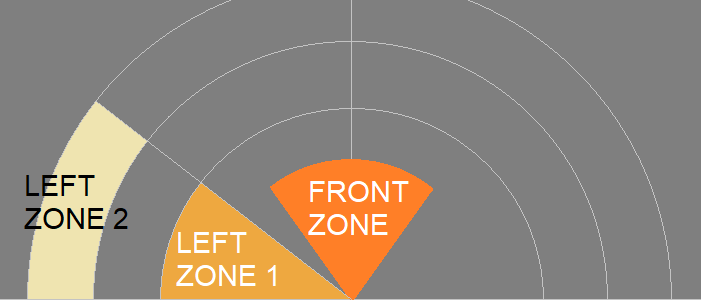
\includegraphics[width=1\linewidth]{rys/autodrive-zones.png}
	\caption{Strefy algorytmu jazdy autonomicznej}
	\label{fig:autodrive-zones}
\end{figure}

Należy zwrócić uwagę, że  Rys. \ref{fig:autodrive-zones} ma charakter poglądowy i nie jest wykonany w skali. Platforma znajduje się tutaj w punkcie środkowym układu współrzędnych, rysunek przedstawia zakres kątów od 0 do 180 stopni, liczonych od kierunku prawego przeciwnie do ruchu wskazówek zegara. W tej samej kolejności przedstawiane są dane zeskanowane przez robota.
\\
Wymiary stref zostały dobrane metodą prób i błędów, dostrajane do momentu w którym robot był w stanie samodzielnie okrążyć pokój bez wjeżdżania w przeszkody.
Wielkości kroków to kolejne z parametrów którymi można regulować jakość pracy algorytmu. Rys. \ref{fig:autodrive-algorithm} prezentuje jego funkcjonowanie w oparciu o wymienione poniżej wartości.

\begin{itemize}
    \item zakres kątów obejmujących strefę \emph{F} to <70, 110>
    \item zakres kątów obejmujących strefy \emph{L1} i \emph{L2} to <140, 180>
    \item promień strefy \emph{F} wynosi 30 cm
    \item promień strefy \emph{L1} wynosi 50 cm
    \item strefa \emph{L2} jest wycinkiem zaczynającym się od promienia równego 70 cm, kończąca się na 90 cm
    \item mały krok jazdy do przodu wynosi 10 cm
    \item mały krok obrotu wynosi 10 stopni
    \item duży krok obrotu wynosi 30 stopni
\end{itemize}

\begin{figure}[ht]
	\centering
		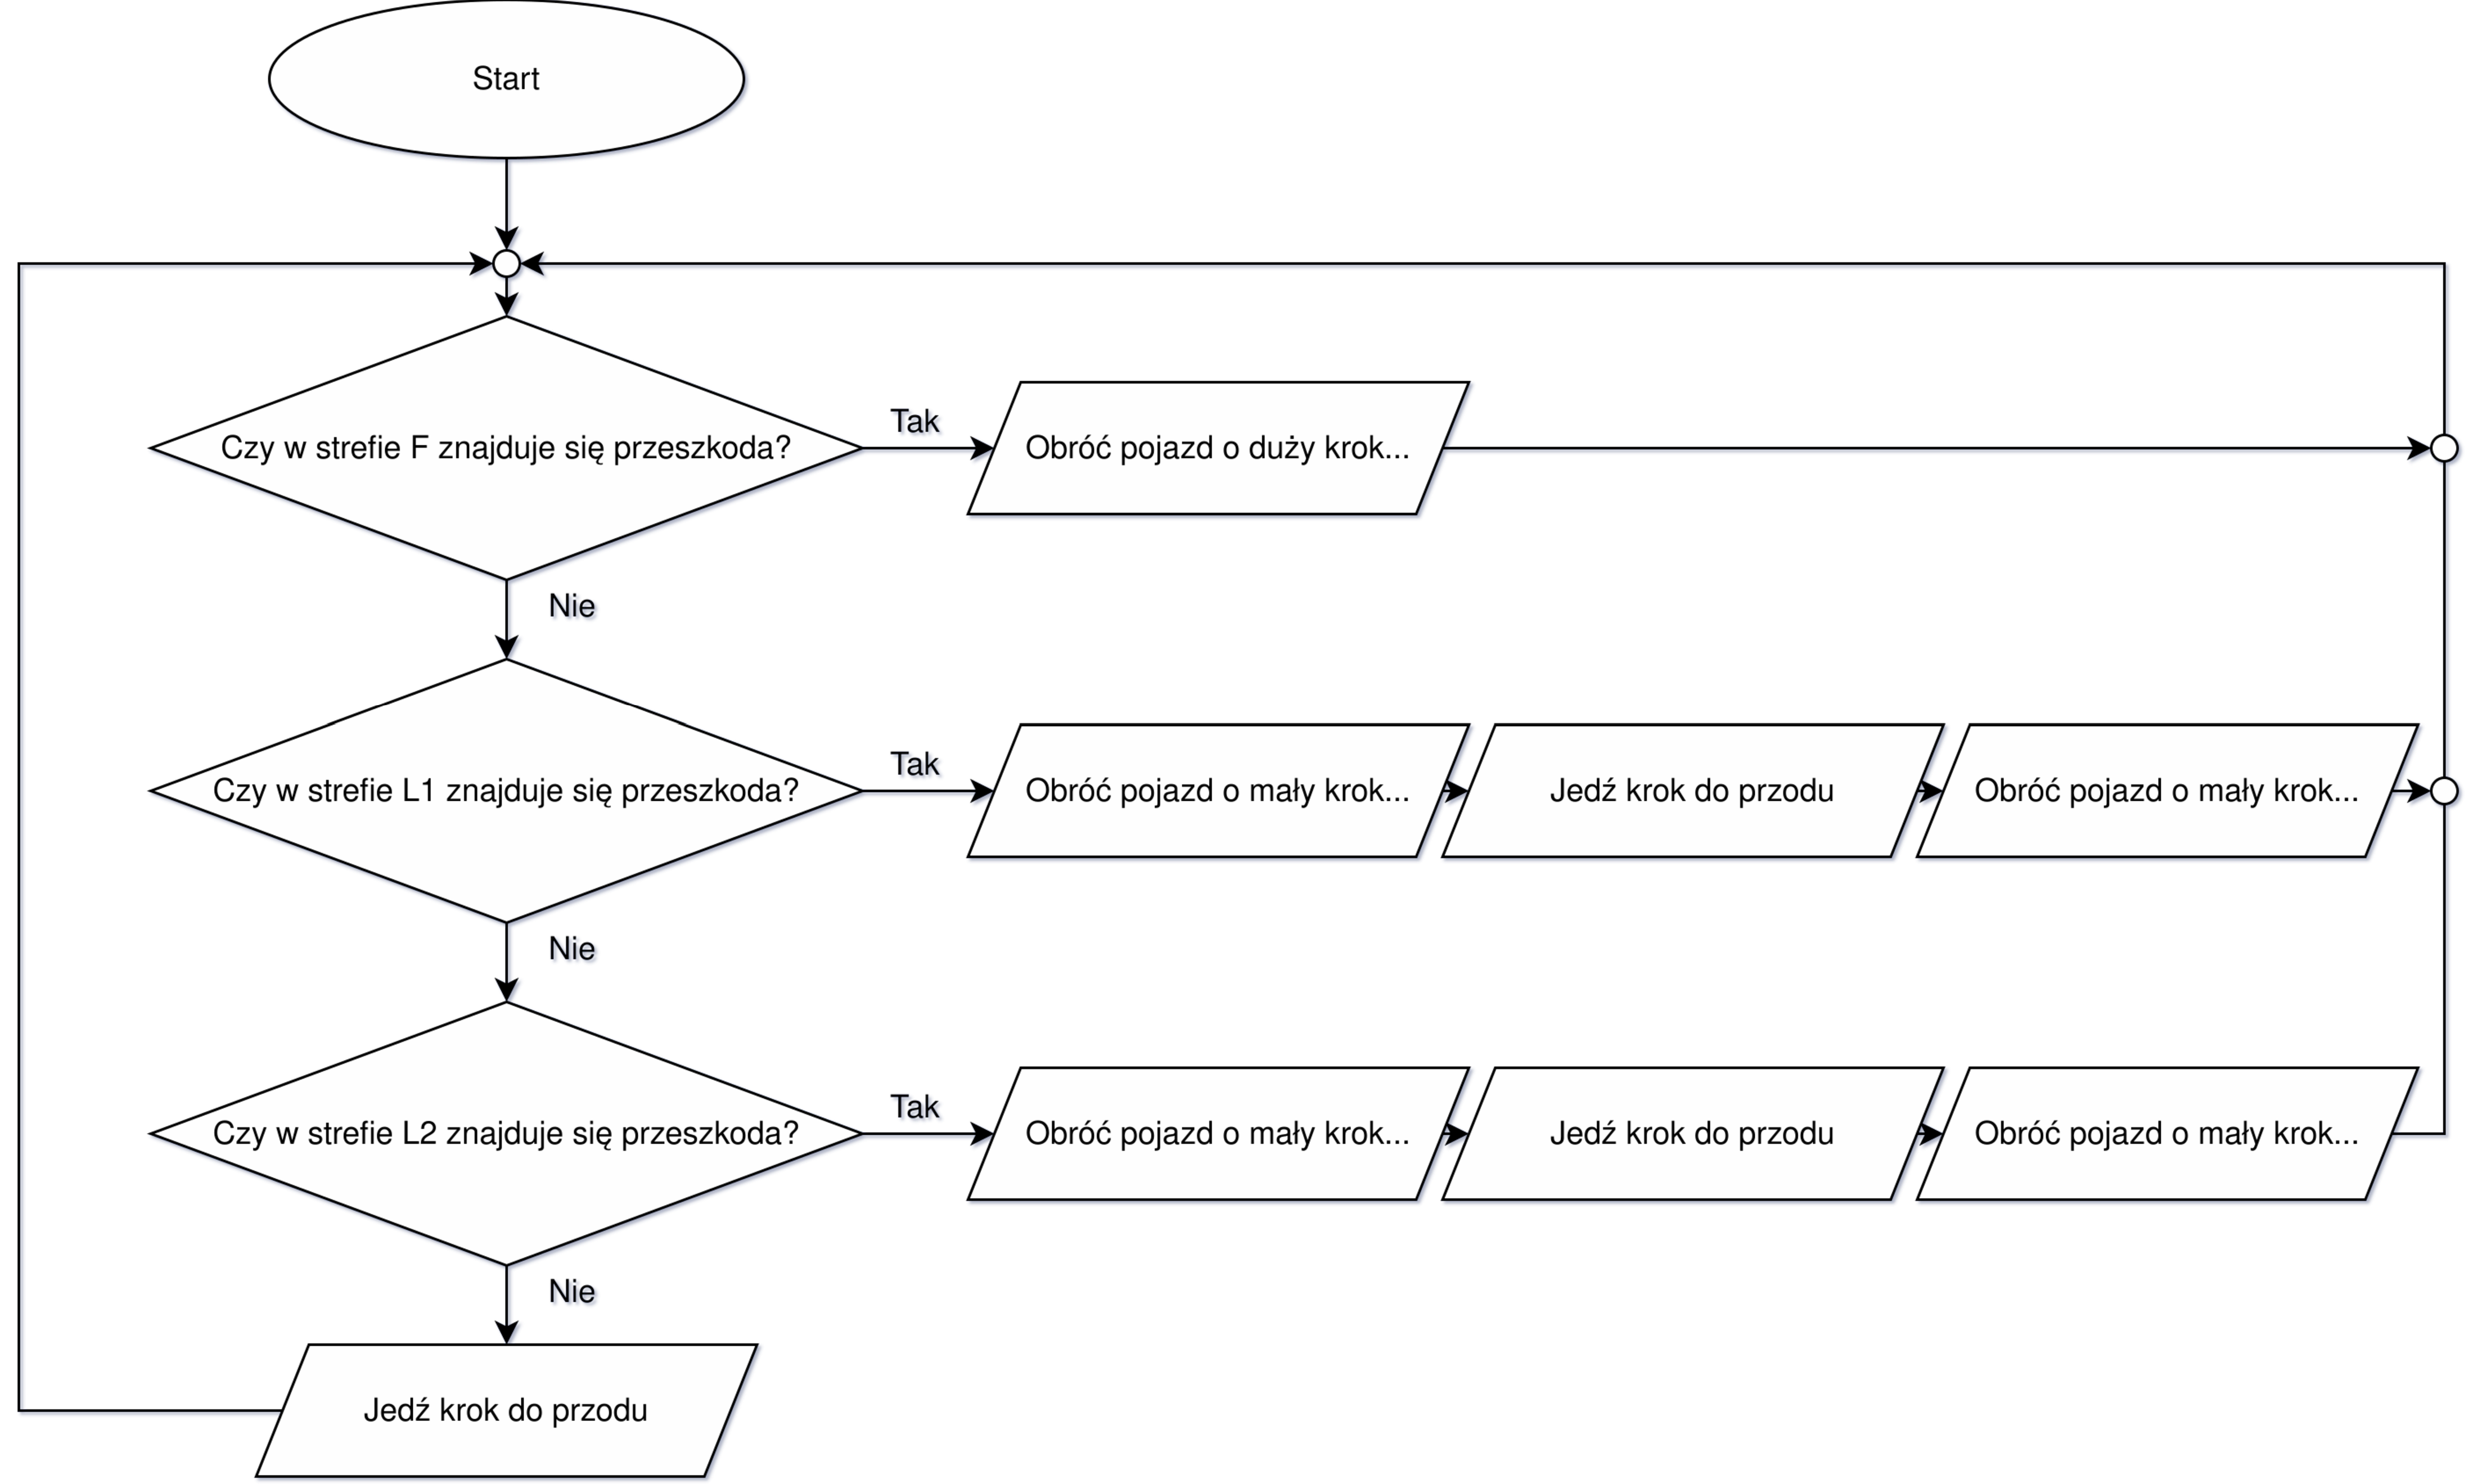
\includegraphics[width=1\linewidth]{rys/autodrive-algorithm.pdf}
	\caption{Algorytm jazdy autonomicznej}
	\label{fig:autodrive-algorithm}
\end{figure}

\section{Firmware}
\label{sec:firmware}
Dzięki zastosowaniu mikrokontrolera jako jednostki sterującej mobilną platformą skanującą zużycie prądu jest bardzo małe (bez peryferiów zużywa <51mA\cite{stm32-datasheet}). Nakłada to niestety ograniczenia związane z mocą obliczeniową urządzenia i dostępną pamięcią w której przechowywany jest program. 

Pierwszym kierunkiem w którym udał się autor były popularne dziś płytki Arduino\cite{arduino-boards}, czego głównym powodem jest łatwość szybkiego prototypowania i szeroki wachlarz gotowych rozwiązań obsługujących różne sensory, serwomechanizmy, wyświetlacze i wiele innych. Płytka nie powinna być zbyt duża, dlatego na uwadze były mniejsze egzemplarze takie jak np. Arduino Nano. Jednak ze względu na niskie taktowanie procesora (16MHz) i niewiele pamięci Flash (32kB) na program wybrana została alternatywa - tzw. płytka ``blue pill``\cite{bluepill}. Jest to nieoficjalna płytka, podobna do Arduino. Można ją zaś programować w tym samym środowisku i wykorzystywać wiele (choć nie wszystkie) z bibliotek napisanych pod oficjalnie wspierane płytki. Jest tak dzięki zestawowi bibliotek STM32duino \cite{stm32duino-github} zapewniających kompatybilność z wcześniej wspomnianym środowiskiem. Do kompilacji i wgrania programu zostało wykorzystane kompatybilne z Arduino - PlatformIO IDE \cite{platformio}.
\\

Program działający na platformie wykonuje jedynie proste polecenia odebrane od aplikacji sterującej i odpowiada prostym potwierdzeniem, wartością lub listą wartości. Poniżej wylistowano polecenia:

\begin{enumerate}
    \item \emph{DRIVE} - ustaw zadaną prędkość na gąsienicach
    \item \emph{ROTATE\_TOWER} - obróć wieżyczkę na żądaną pozycję
    \item \emph{KILL} - odłącz sygnał sterujący od serwomechanizmów
    \item \emph{PRINT} - pokaż tekst na wyświetlaczu
    \item \emph{BEEP} - wydaj serię dźwięków o zdefiniowanej liczbie i czasie trwania
    \item \emph{GET\_MAG} - zwróć surowy pomiar z osi X i Y magnetometru
    \item \emph{GET\_AZIMUTH} - zwróc azymut w którym skierowany jest robot
    \item \emph{GET\_DISTANCE} - zmierz odległość od przeszkody
    \item \emph{GET\_TIME} - zwróć wartość czasu w milisekundach od uruchomienia robota
    \item \emph{MOVE} - przemieść się o zadany dystans do przodu lub do tyłu
    \item \emph{ROTATE\_TO} - obróć się na zadany azymut
    \item \emph{ROTATE} - obróć się o kąt
    \item \emph{SCAN} - skanuj otoczenie
    \item \emph{SET\_MAG\_CAL} - ustaw wartości do kalibracji magnetometru
    \item \emph{GET\_MAG\_CAL} - pobierz wartości kalibracji
    \item \emph{RESET} - uruchom ponownie robota
\end{enumerate}



\section{Schemat budowy mechanicznej}
Główną przeszkodą w nawigacji zliczeniowej jest kumulujący się błąd. Wynika on z czynników niemożliwych do zwalczenia w całości, które są naturalne w każdym fizycznym obiekcie. Do tych czynnikó

\begin{figure}[ht]
	\centering
		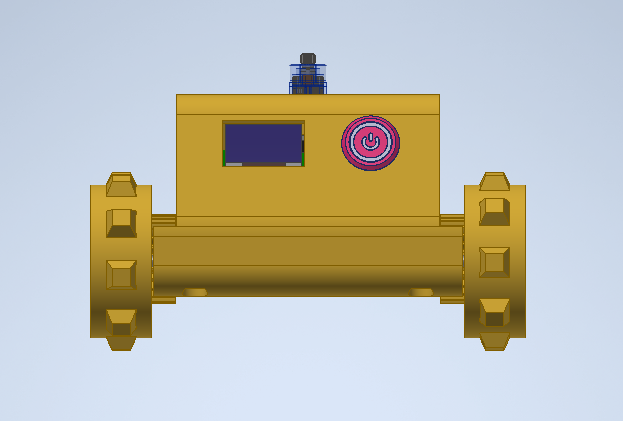
\includegraphics[width=0.5\linewidth]{rys/view1.png}
	\caption{Rzut główny platformy}
	\label{fig:view1}
\end{figure}

\begin{figure}[ht]
	\centering
		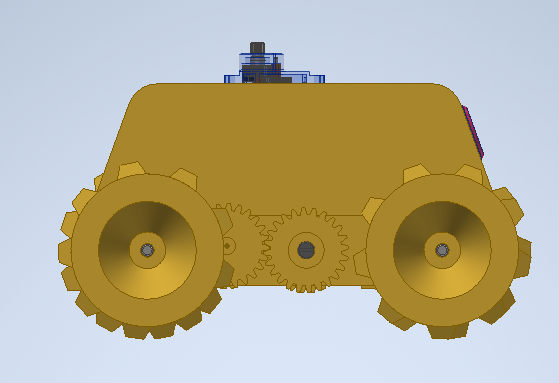
\includegraphics[width=0.5\linewidth]{rys/view2.png}
	\caption{Rzut platformy z prawej strony}
	\label{fig:view2}
\end{figure}

\begin{figure}[ht]
	\centering
		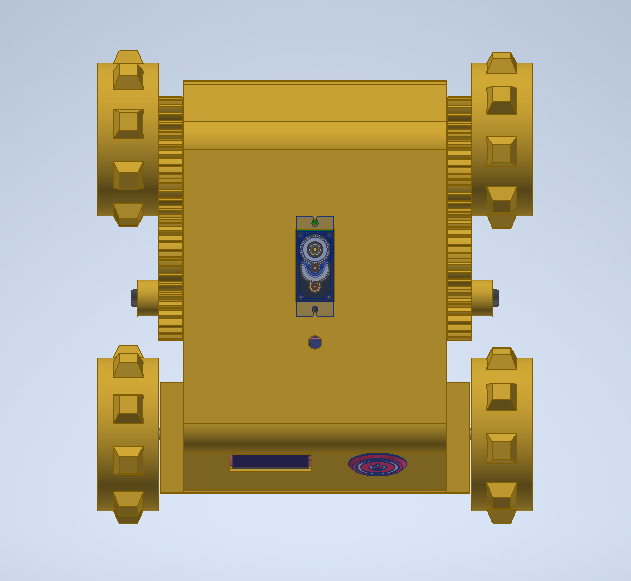
\includegraphics[width=0.5\linewidth]{rys/view3.png}
	\caption{Rzut platformy z góry}
	\label{fig:view3}
\end{figure}

\begin{figure}[ht]
	\centering
		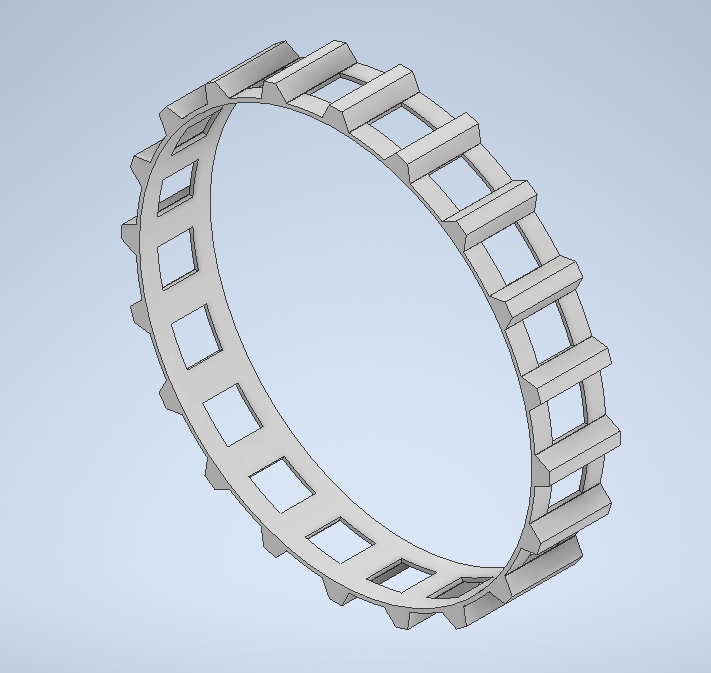
\includegraphics[width=0.5\linewidth]{rys/tracks-final.png}
	\caption{Rzut izometryczny gąsienicy}
	\label{fig:tracks}
\end{figure}


\section{Schemat elektroniczny}
%[>TODO wspomnij o sensorach ultradzw oraz sharp IR]



\chapter{Ewaluacja}
\label{sec:evaluation}

Poniższy rozdział opisuje sposób w jaki sposób w ramach powstałego projektu przebiegają procedury mające na celu stworzenie możliwie najbardziej oddającej rzeczywistość mapy pomieszczenia. Autor przedstawia problemy które napotkał dążąc do celu, ich genezę oraz konieczne zmiany i udoskonalenia. Również przybliżone zostały aspekty korzystania z poszczególnych dostępnych funkcjonalności.

Aby rozpocząć proces ewaluacji i udoskonalania projektu robot powinien mieć zapewnione stabilne połączenie z komputerem na którym pracuje środowisko sterujące. W tym celu po otwarciu okna głównego aplikacji należy skorzystać z opisanej wcześniej sekcji \emph{CONNECTION} uprzednio łącząc elementy systemu w sposób przedstawiony na rysunku \ref{fig:pc-bt-connection}. Następnie należy wybrać odpowiedni port szeregowy i kliknąć przycisk służący do nawiązania połączenia. Po kilku sekundach, jeżeli procedura przebiegła pomyślnie, platforma wyda trzy krótkie sygnały dźwiękowe - oznacza to gotowość do przyjmowania poleceń.

\begin{figure}[ht]
	\centering
		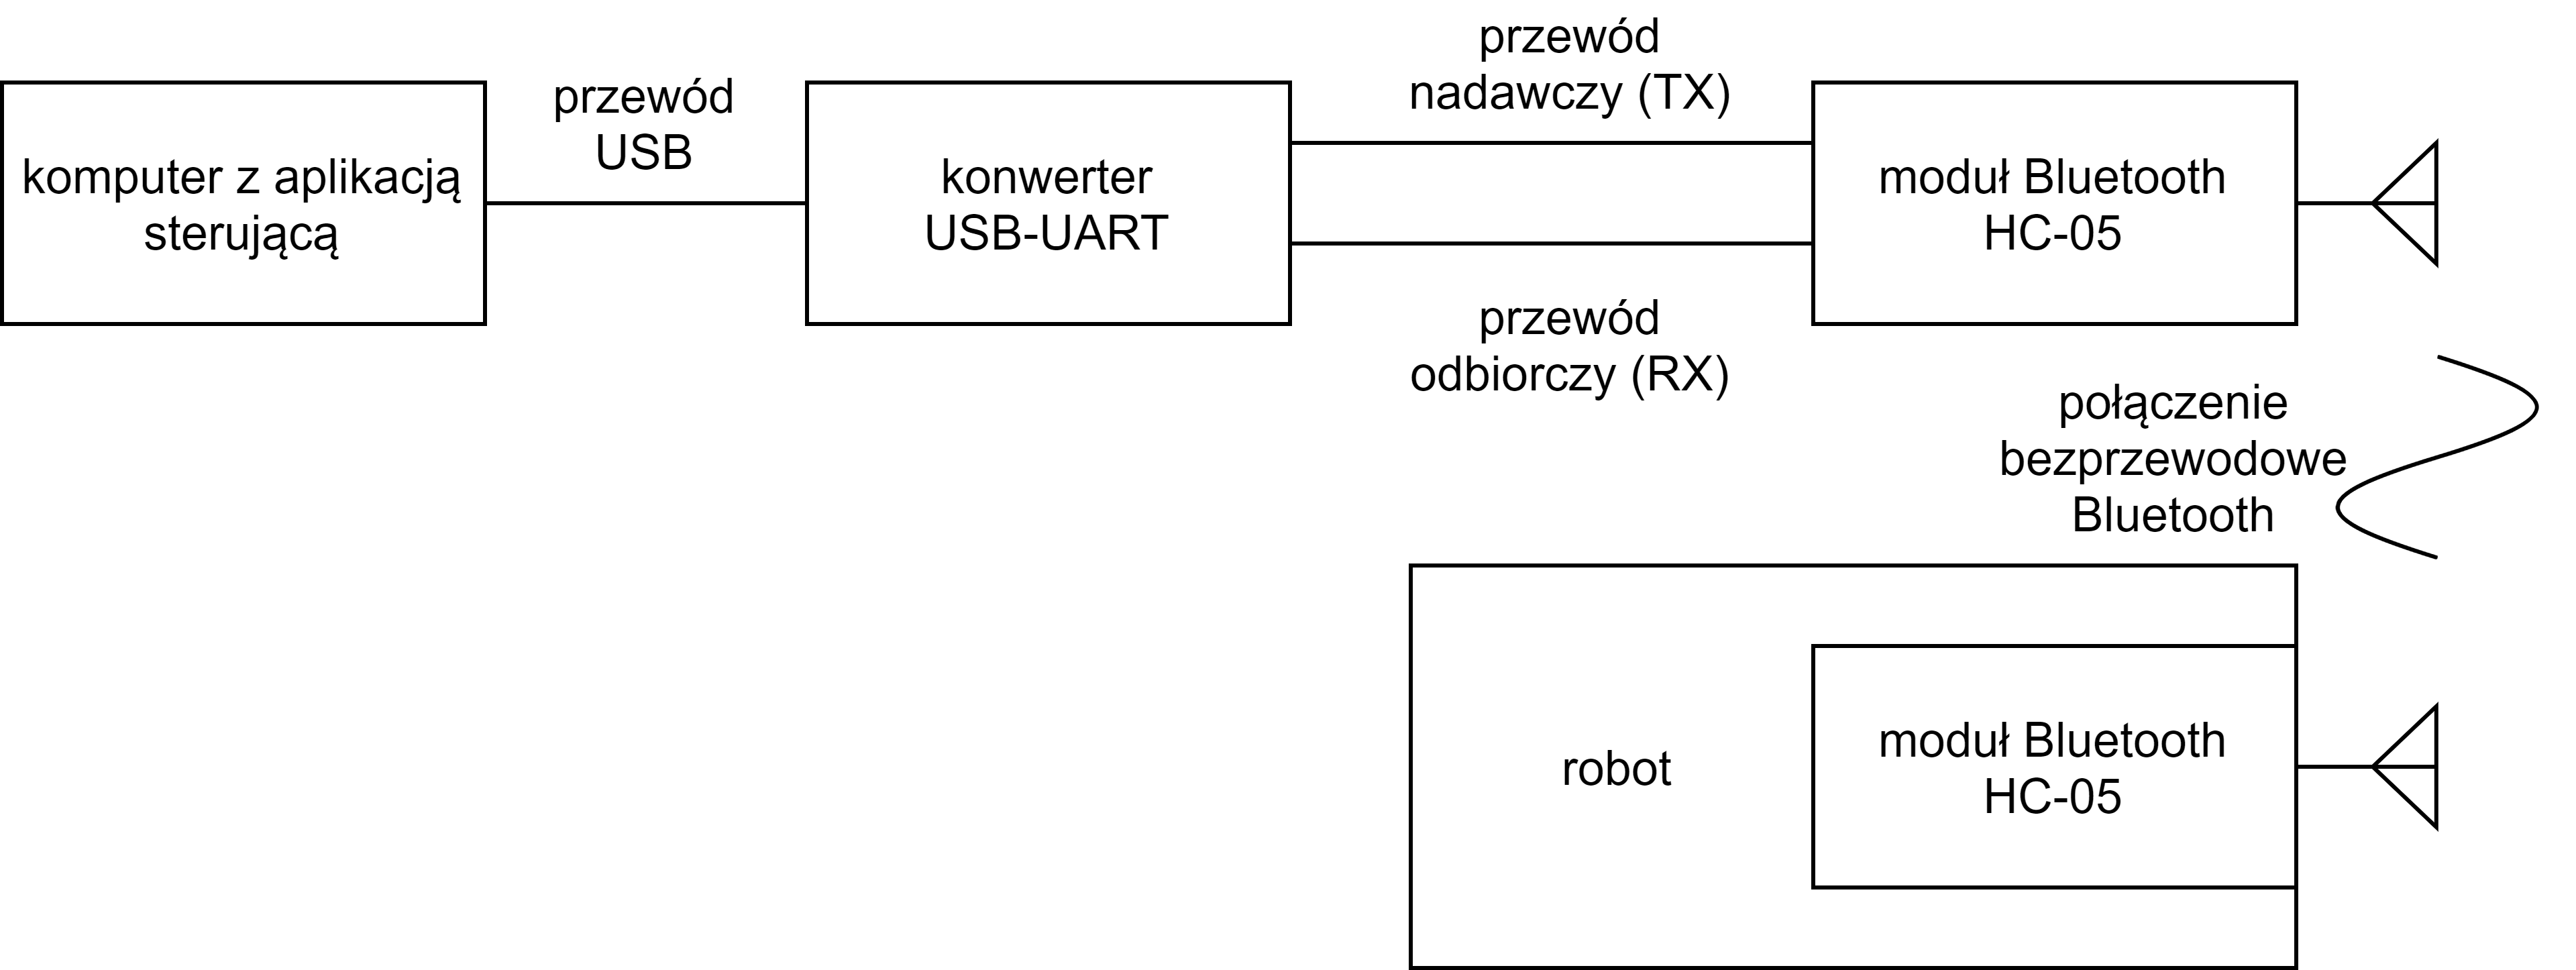
\includegraphics[width=1\linewidth]{rys/pc-bluetooth-robot connection.png}
	\caption{Schemat połączenia z robotem}
	\label{fig:pc-bt-connection}
\end{figure}

Opisana procedura jest konieczna przy każdym uruchomieniu systemu. Mając to na uwadze, można przystąpić do ewaluacji opisanej w kolejnych rozdziałach.

\section{Odometria}
\label{sec:odometry}
Robot korzysta z nawigacji zliczeniowej w celu połączenia pomiarów odległości zebranych z otoczenia i aproksymacji ich położenia na płaszczyźnie względem jednego ustalonego punktu. Zliczaniu podlegają dwie wartości - dystans przejechany wzdłuż oraz obrót pojazdu w miejscu. Szereg zmierzonych w ten sposób wartości umożliwia odtworzenie przejechanej ścieżki. Rysunek \ref{fig:odom-axis-simplified} przedstawia rzeczywisty oraz uproszczony model podwozia robota. X na rysunku oznacza środek robota - pionową oś wokół której się obraca. Zamiast uwzględniać obie poziome osi i 4 koła, upraszcza się go do formy robota o jednej osi, z jedną parą kół. Gdy oba koła poruszają się w tę samą stronę, robot przesuwa się w przód lub w tył. Gdy pracują przeciwbieżnie - obraca się wokół osi oznaczonej X.  

\begin{figure}[H]
	\centering
		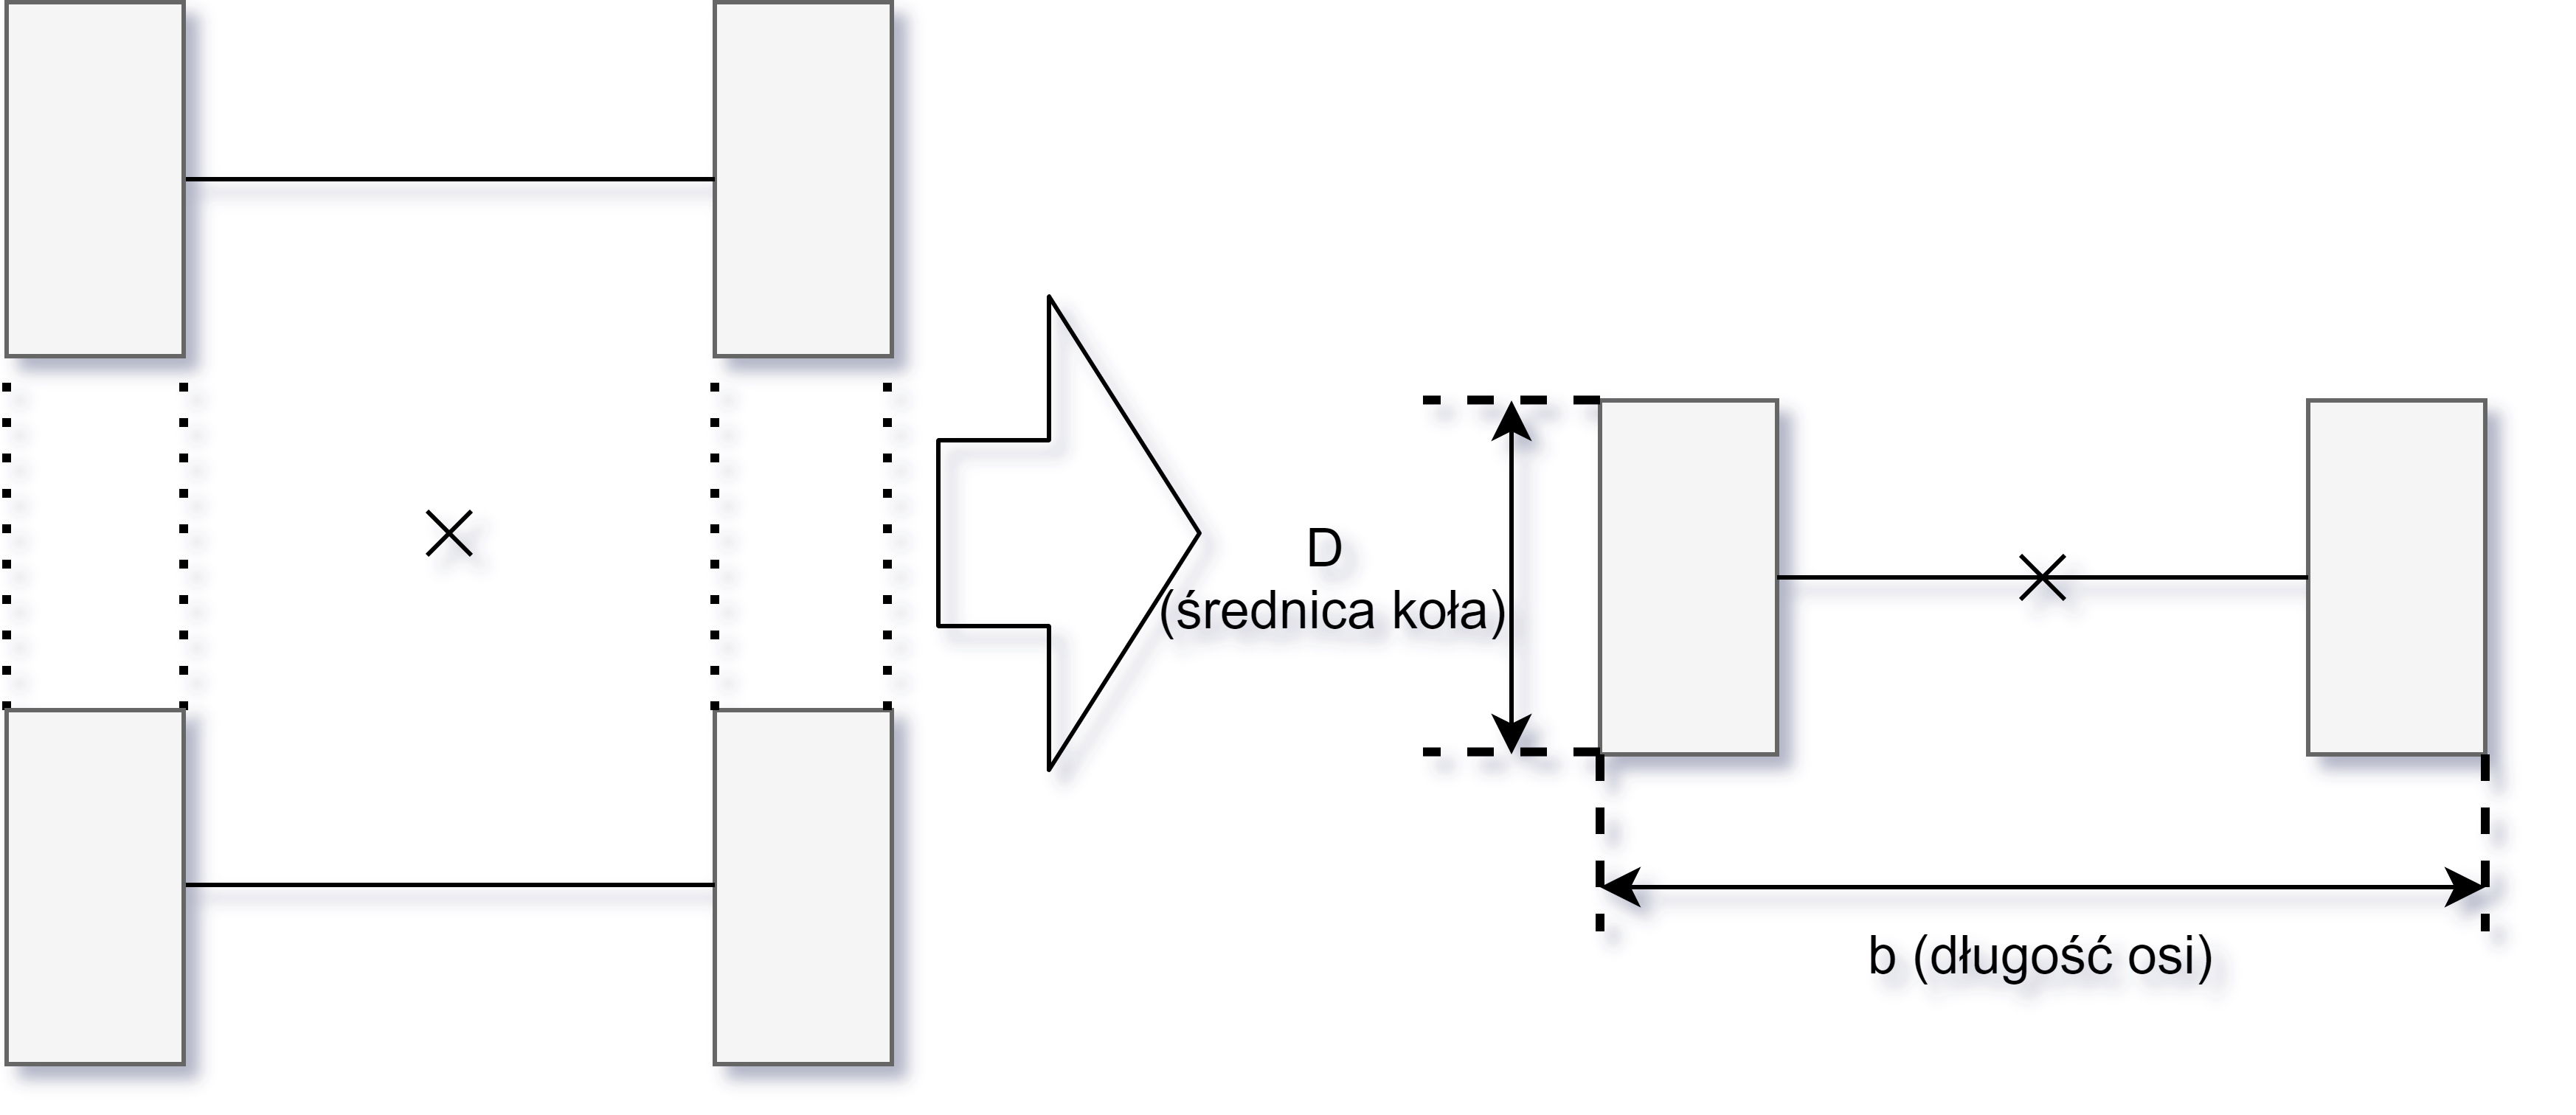
\includegraphics[width=0.8\linewidth]{rys/robot-odometry-simplified.png}
	\caption{Model rzeczywisty i uproszczony }
	\label{fig:odom-axis-simplified}
\end{figure}


Pierwszym pomysłem było wykorzystanie enkoderów do pomiaru translacji pojazdu wzdłuż jego osi ruchu, pozostawiając zliczanie obrotu funkcjom korzystającym z magnetometru.

\begin{figure}[H]
	\centering
		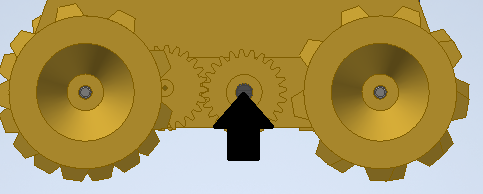
\includegraphics[width=0.6\linewidth]{rys/encoder-position.png}
	\caption{Umiejscowienie enkodera z prawej strony robota}
	\label{fig:encoder-pos}
\end{figure}

Enkodery zostały zamontowane w miejscu przedstawionym na rysunek \ref{fig:encoder-pos}, symetrycznie po obu stronach podwozia. Napęd podany od serwomechanizmu przez przekładnię zębatą przenosi napęd zarówno na tylne koło jak i enkoder, z przekładniami 1:1 w obu przypadkach. Dzięki takiemu rozwiązaniu pełny obrót enkodera odpowiada pełnemu obrotowi koła. Enkoder obrotowy EC-11 generuje 20 impulsów przy kącie obrotu 360°. Aby można było wyznaczyć pokonaną odległość, w pierwszej kolejnosci należy obliczyć stosunek ilości impulsów do przejechanego dystansu - w tym celu autor stworzył prosty wzór (\ref{eq:dpr}).

\begin{equation}
    DPR = \frac{2 \pi r}{p}
    \label{eq:dpr}
\end{equation}
DPR - współczynnik (ang. Distance to Pulse Ratio) wyrażany w cm/impuls \\
r - promień koła pojazdu \\
p - liczba impulsów enkodera na obrót koła \\ \\

Wiedząc ile impulsów generuje enkoder, oraz znając wymiary koła w łatwy sposób można obliczyć DPR, co uczyniono poniżej (\ref{eq:dpr2}).

\begin{equation}
\begin{aligned}
    DPR = \frac{2 \pi 2,5cm}{20imp} \\[5pt]
    DPR = 0.785 \frac{cm}{imp} \\[5pt]
    \frac{1}{DPR} = 1.274
\end{aligned}
\label{eq:dpr2}
\end{equation}

Znając współczynnik aby obliczyć przejechany dystans wystarczy zmierzyć liczbę impulsów jakie wystąpiły podczas przejazdu a następnie pomnmożyć je przez DPR. Otrzymany wynik oznacza przesunięcie robota wyrażone w centymetrach. Jako że platforma posiada dwa enkodery, a nie jest możliwe zachowanie idealnie prostego toru jazdy, wyciągana jest średnia liczba impulsów. Ze względu na grubość i wypustki na gąsienicach oraz ich poślizg rzeczywisty dystans przejechany będzie inny od zadanego. Dla kompensacji tej różnicy wartość DPR została skorygowana ręcznie do takiej, przy której błąd przemieszczenia robota zawierał się w granicy ±10\% na zadanym dystansie 100cm. Widoczna w kodzie programu, skorygowana wartość $\frac{1}{DPR}$ wynosi $1.325$ co odpowiada $DPR=0.755$ . Listing \ref{lst:move} prezentuje funkcję realizującą to zadanie.

\begin{listing}[ht]
\begin{minted}[fontsize=\footnotesize]{c++}
//MOVE
case 9:
{
    reset_encoders();
    float val = getArgument(command, 1).toInt() * 1.325;

    if (val > 0)
        driveMotors(90, 90);
    else
        driveMotors(-90, -90);

    val = abs(val);
    while ((left_encoder_counter + right_encoder_counter) / 2 < val)
    {
    }

    driveMotors(0, 0);
    delay(100);
    Serial2.println("OK");
}
\end{minted}
\caption{Fragment kodu obsługującego polecenie \emph{MOVE}}
\label{lst:move}
\end{listing}



Podczas wykonywania polecenia \emph{MOVE} na gąsienice zadawana jest pełna prędkość i w pętli sprawdzana jest średnia liczba impulsów wygenerowanych przez enkoder. Dla optymalizacji algorytmu, zamiast przeliczać przy każdym pomiarze liczbę impulsów razy wartość DPR, na początku zadana w parametrze wartość odległości jest mnożona przez $\frac{1}{DPR}$, i dalej w takiej formie ta wartość wykorzystywana przy operacji porównania. W momencie w którym średnia zliczona liczba impulsów przekroczy jej wartość, serwomechanizmy zostają zatrzymane.
\\ 

Obrót (funkcja \emph{ROTATE}) polega na zadaniu przeciwstawnych wartości prędkości na obie gąsienice. W celu obrotu poruszają się one przeciwbieżnie, z równymi prędkościami. Pierwsza implementacja funkcji obrotu wyglądała jak przedstawiono poniżej:

\begin{listing}[ht]
\begin{minted}[fontsize=\footnotesize]{c++}
void rotateTo(int azimuth)
{
    if (calcAngleDistance(getAzimuth(), azimuth) > 0)
        driveMotors(-90, 90);
    else
        driveMotors(90, -90);

    while (true)
    {
        if (abs(calcAngleDistance(getAzimuth(), azimuth)) <= 10)
            break;
        delay(10);
    }
    driveMotors(0, 0);
    delay(100);
}
\end{minted}
\caption{Funkcja będąca głównym elementem obsługi poleceń \emph{ROTATE} oraz \emph{ROTATE\_TO}}
\label{lst:rotate-to-function}
\end{listing}

Na początku mierzony jest azymut początkowy i obliczany jest azymut końcowy (tj. początkowy + zadana wartość obrotu). Dalej wykonywana jest ta sama funkcja co w przypadku \emph{ROTATE\_TO} przyjmująca parametr azymutu końcowego. Podczas obrotu, w pętli, sprawdzana jest różnica kąta aktualnego od zadanego. Jeżeli wartość bezwzględna obrotu znajdzie się w zakresie ±10° robot zatrzyma się.

Takie rozwiązanie jest dobre, o ile magnetometr jest skalibrowany i funkcjonuje poprawnie. Niestety, podczas skanów okazało się że nie można polegać na pomiarach z tego sensora - więcej o tym znajduje się w sekcji \ref{sec:scan}. Z tego powodu koniecznym okazała się zmiana podejścia do pomiaru obrotu.

Listing \ref{lst:rotate} przedstawia nowe podejście osbługi polecenia \emph{ROTATE}. Jest ono mniej dokładne od poprzedniego, bardziej podatne na dryf (błąd obrotu kumuluje się), natomiast taki pomiar jest odporny na zakłócenia pola magnetycznego.
Tym razem procedura jest analogiczna jak w przypadku ewaluacji polecenia \emph{MOVE}. W pętli sprawdzana jest średnia liczba impulsów, jednak tym razem gąsienice poruszają się przeciwbieżnie. Kąt obrotu na początku należy przemnożyć przez pewien współczynnik tak aby odpowiadał on ilości impulsów. Platforma kończy ruch w momencie gdy średnia wartość przekroczy obliczony próg impulsów.


\begin{listing}[ht]
\begin{minted}[fontsize=\footnotesize]{c++}
// ROTATE
    case 11:
    {
        reset_encoders();
        float val = getArgument(command, 1).toInt() * 0.164;
        if (val > 0)
            driveMotors(-90, 90);
        else
            driveMotors(90, -90);

        val = abs(val);
        while ((left_encoder_counter + right_encoder_counter) / 2 < val)
        {
        }

        delay(100);
        driveMotors(0, 0);
        Serial2.println("OK");
    }
    break;
\end{minted}
\caption{Nowa implementacja obsługi polecenia \emph{ROTATE}}
\label{lst:rotate}
\end{listing}

Stosunek kąta obrotu do liczby impulsów ($0.164$) został wyznaczony eksperymentalnie. Najpierw przyjęto wartość 1. Następnie zadawany był kąt obrotu 90°, po czym mierzony był rzeczywisty kąt obrotu. Jeżeli wynosił on więcej, współczynnik redukowano o 0,1; analogicznie gdy obrót był mniejszy niż zadano. Gdy tak zgrubna regulacja była niewystarczająca (albo za mały albo za duży obrót), krok został zmniejszony do 0,05. Po kolejnej zmianie kroku do 0,02 czynność powtarzano do momentu w którym dalsza korekcja nie była konieczna. \\

Taka implementacja została zachowana do końca projektu. Polecenie \emph{ROTATE\_TO} dalej korzysta ze starego sposobu z użyciem magnetometru, jednak nie jest ono wykorzystywane podczas pomiarów.

\subsection{Kalibracja magnetometru}
\label{sec:mag-cal}
Wykorzystywany w projekcie moduł magnetometru jest urządzeniem czułym i bardzo podatnym na zakłócenia - szczególnie jeśli mierzone jest pole magnetyczne ziemi. Poza zakłóceniami z otoczenia, występują również te wynikające z samej budowy robota - wszelkie przewody przez które płynie prąd generują swoje własne pola, nawet same metalowe elementy interferują z pomiarem. Na te zakłócenia należy zwrócić uwagę i podjąć kroki mające na celu ich kompensację. Warto też wspomnieć, że w tej pracy jednostki uzyskane z pomiaru nie mają znaczenia - jedyne co jest potrzebne w celu uzyskania informacji o kierunku w którym robot jest zwrócony to kierunek i zwrot zmierzonego wektora wartości natężenia pola.

Pierwszym problemem są zakłócenia typu \emph{hard iron}. Ich obecność przejawia się w postaci stałego przesunięcia mierzonych we wszystkich trzech osiach wartości natężenia pola magnetycznego. Zmierzone wartości można przedstawić na trójwymiarowym wykresie (jak uczyniono w pierwszych wersjach aplikacji sterującej). Każda z osi wykresu odpowiada osi pomiaru natężenia pola magnetycznego. W idealnej sytuacji zbór punktów powinien być osadzony na sferze o środku w punkcie $(0,0,0)$. Tak się jednak nie dzieje, co jest widoczne na rysunku \ref{fig:3d-mag-no-cal}.

\begin{figure}[ht]
	\centering
		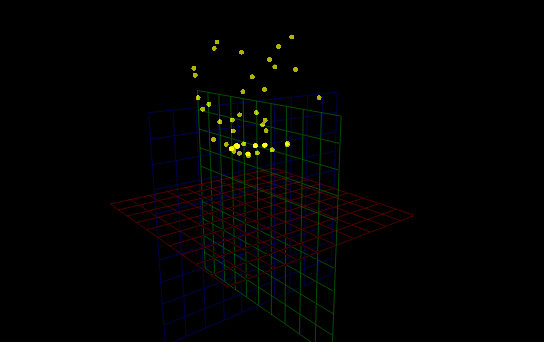
\includegraphics[width=0.6\linewidth]{rys/ScanBot-03-magnetometer-3d-decalibrated.PNG}
	\caption{Wykres obrazujący dane pozyskane z nieskalibrowanego magnetometru}
	\label{fig:3d-mag-no-cal}
\end{figure}

Aby dokonać korekcji \emph{hard iron} \cite{hard-iron}\cite{hard-soft-iron} dla każdej osi z osobna należy wyznaczyć minimalną i maksymalną zmierzoną wartość. Sumę obu wartości dzieli się przez 2, a uzyskana liczba to przesunięcie (ang. \emph{offset}). Aplikacja korekcji polega na odjęciu tej liczby od zmierzonej wartości.
Tą procedurę dla trzech osi przedstawiają kolejno rysunki \ref{fig:3d-mag-hard-corr-x}, \ref{fig:3d-mag-hard-corr-y} i \ref{fig:3d-mag-hard-corr-z}.

\begin{figure}[H]
	\centering
		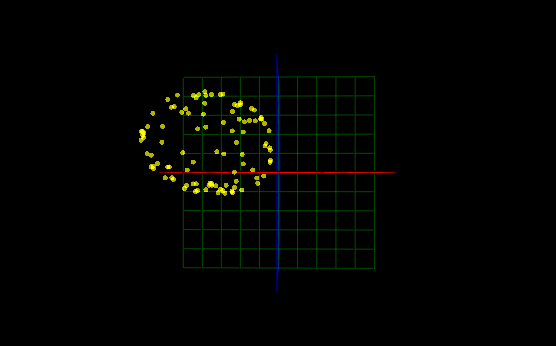
\includegraphics[width=0.6\linewidth]{rys/ScanBot-04-magnetometer-3d-calibration.PNG}
	\caption{Korekta przesunięcia \emph{hard iron} dla osi X}
	\label{fig:3d-mag-hard-corr-x}
\end{figure}

\begin{figure}[H]
	\centering
		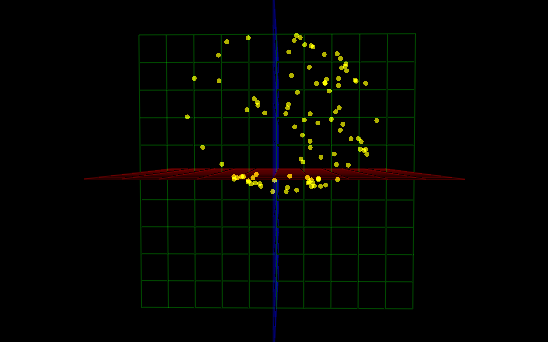
\includegraphics[width=0.6\linewidth]{rys/ScanBot-05-magnetometer-3d-calibration.PNG}
	\caption{Korekta przesunięcia \emph{hard iron} dla osi Y}
	\label{fig:3d-mag-hard-corr-y}
\end{figure}

\begin{figure}[H]
	\centering
		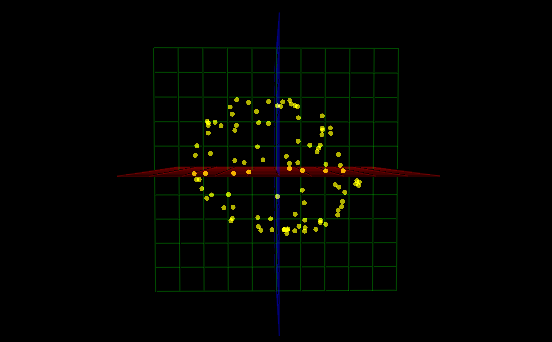
\includegraphics[width=0.6\linewidth]{rys/ScanBot-06-magnetometer-3d-calibration.PNG}
	\caption{Korekta przesunięcia \emph{hard iron} dla osi Z}
	\label{fig:3d-mag-hard-corr-z}
\end{figure}

Niestety, kształt chmury punktów wciąż daleki jest od idealnej sfery. Efektem tego jest nieliniowość uzyskanego azymutu - zmiana rzeczywistego kąta skierowania platformy względem zmiany zmierzonej będzie się znacząco różniła w zależności od początkowej pozycji. Ten efekt można by obejść za pomocą mapowania wartości za pomocą funkcji odpowiedniej krzywej, jednak wymagałoby to formułowania skomplikowanego równania, bądź wyznaczenia arbitralnego przebiegu funkcji. Istnieje jednak mniej wymagające obliczeniowo podejście z zastosowaniem rachunku macierzowego \cite{hard-soft-iron}. Dla uproszczenia obliczeń, zrezygnowano z pomiaru w trzech osiach, zamiast tego mierzone są jedynie natężenia pola w osiach X i Y (rysunek \ref{fig:2d-mag-no-cal}).

\begin{figure}[H]
	\centering
		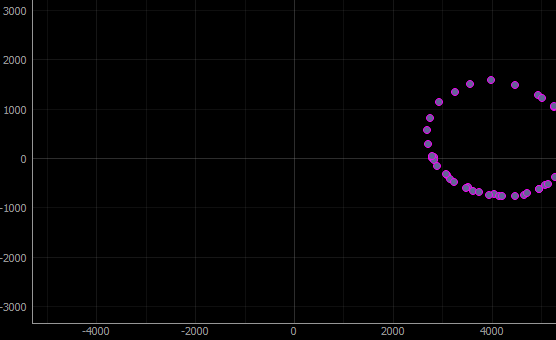
\includegraphics[width=0.6\linewidth]{rys/ScanBot-08-2d-calibration-theta-sigma.PNG}
	\caption{Rozkalibrowany magnetometr na dwuwymiarowej płaszczyźnie}
	\label{fig:2d-mag-no-cal}
\end{figure}

Tak jak w przypadku trzech wymiarów, w pierwszej kolejności dokonywana jest korekcja zniekształceń \emph{hard iron} na wszystkich osiach (rysunek \ref{fig:2d-mag-hard-corr-xy}).

\begin{figure}[H]
	\centering
		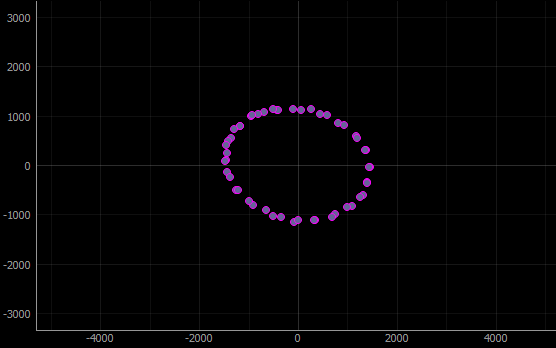
\includegraphics[width=0.6\linewidth]{rys/ScanBot-10-2d-calibration-theta-sigma-2-added-hard-offset-reset-data-so-soft-iron-values-are-proper.PNG}
	\caption{Korekcja hard iron}
	\label{fig:2d-mag-hard-corr-xy}
\end{figure}


Teraz można przystąpić do procedury kompensacji zniekształceń \emph{soft iron}. Idealnie, po dokonaniu korekcji w dwóch wymiarach, punkty na wykresie można by umieścić na okręgu - tak jednak nie jest. Uzyskany kształt bardziej przypomina elipsę, i ta właściwość zostanie wykorzystana. Przebieg procesu przedstawiono w formie pseudokodu (Algorytm \ref{pcode:soft-iron-corr}).

\begin{algorithm}[H]
\SetAlgoLined
\SetAlgorithmName{Algorytm}{}\\

// Lista zmierzonych punktów w postaci par współrzędnych $(P_{_x}, P_{_y})$ \\
$P$ \\
// Lista do której dodane zostaną odległości od $(0,0)$ do $P$ \\
$r$ \\[10pt]

// Oblicz odległości punktów od środka układu współrzędnych \\ 
\For{$i = 0, ..., 180$}{
$r_{i} = \sqrt{ P_{i_x}^2 + P_{i_y}^2 }$
}
\EndFor \\[10pt]

// Wartości $P_{min}$ i $P_{max}$ odpowiadają kolejno końcom półosi małej i półosi wielkiej elipsy. \\ 
$r_{min} = min(r)$ \\ 
$r_{max} = max(r)$ \\ 
$P_{min} = min(P)$ \\ 
$P_{max} = max(P)$ \\[10pt]

// Oblicz kąt obrotu elipsy \\ 
$\theta = arctan2(P_{max_y}, P_{max_x})$ \\[10pt]

// Wyznacz macierz $R$ \\
$R = \begin{bmatrix}
    cos\theta & sin\theta\\
    -sin\theta & cos\theta
    \end{bmatrix}$ \\[10pt]

// Oblicz parametr skalujący \\ 
$\sigma = \frac{r_{min}}{r_{max}}$ \\[10pt]

// Lista do której zostaną dodane punkty $P$ po przekształceniu \\
$P2$ \\[10pt]

// Obróć elipsę o kąt -$\theta$ mnożąc punkty przez macierz \\ 
\For{$i = 0, ..., 180$}{
$   
\mathit{P2_{i}}
=
\begin{bmatrix}
    cos\theta & sin\theta\\
    -sin\theta & cos\theta
\end{bmatrix}
\times
\begin{bmatrix}
    \mathit{P}_{i_x}\\
    \mathit{P}_{i_y}
\end{bmatrix}
$
}
\EndFor\\[10pt]

// Lista do której zostaną dodane punkty $P2$ po przeskalowaniu \\
$P3$ \\[10pt]

// Przeskaluj elipsę \\ 
\For{$i = 0, ..., 180$}{
$\mathit{P3}_{i_x} = \mathit{P2}_{i_x} \times \sigma$ \\ 
$\mathit{P3}_{i_y} = \mathit{P2}_{i_y}$ 
}
\EndFor\\[10pt]

// Lista $P3$ zawiera wartości wyjściowe po korekcji \\ 
\caption{Kompensacja zniekształceń \emph{soft iron}}
\label{pcode:soft-iron-corr}
\end{algorithm}

%%%%%%%%%%%%%%%%%%%%%%%%%%%%%%%%%%%%%%%%%%%%%%%%%%%%%%%%%%%%%%%%%%%%%%%%%%%%%%%%%%%%%%%%%%%%%%%%%%%%%%%%
%%%%%%%%%%%%%%%%%%%%%%%%%%%%%%%%%%%%%%%%%%%%%%%%%%%%%%%%%%%%%%%%%%%%%%%%%%%%%%%%%%%%%%%%%%%%%%%%%%%%%%%%
% \begin{enumerate}
%     \item Dla każdego z punktów liczony jest promień $r$ (wektor od $(0,0)$ do danego punktu)
%     \item Wyznaczana jest maksymalna wartość promienia $rmin$ i $rmax$. Te wartości odpowiadają kolejno półosi małej i półosi wielkiej elipsy.
%     \item Dla punktu odpowiadającego promieniowi $rmax$ Obliczany jest kąt $\theta$ za pomocą dwuargumentowej funkcji $arctan2(y,x)$, gdzie $x$ i $y$ są współrzędnymi punktu. Kąt ten odpowiada kątowi obrotu elipsy.
%     \item Tworzona jest macierz $R$. Posłuży do obrotu elipsy.
%     $R = \begin{bmatrix}
%             cos\theta & sin\theta\\
%             -sin\theta & cos\theta
%         \end{bmatrix}$
%     \item Obliczany jest parametr $\sigma$. Posłuży do ściskania elipsy. $\sigma = \frac{rmin}{rmax}$
%     \item Za pomocą macierzy $R$ elipsa jest obracana o kąt -$\theta$ w celu zrównania jej wielkiej półosi z osią OX układu współrzędnych. Współrzędne każdego z punktów kolejno są osobno przekształcane za pomocą mnożenia macierzy:
%     $   
%         \mathit{v}_{2}
%         =
%         \begin{bmatrix}
%             cos\theta & sin\theta\\
%             -sin\theta & cos\theta
%         \end{bmatrix}
%         \times
%         \begin{bmatrix}
%             \mathit{v}_{1x}\\
%             \mathit{v}_{1y}
%         \end{bmatrix}
%     $
%     gdzie $\mathit{v}_{2}$ to wynikowy wektor zawierający współrzędne przekształconego punktu.
%     \item Obróconą elipsę sprowadza się do postaci okręgu poprzez ściśnięcie jej w osi X. Robi się to przemnażając współrzędną x każdego z punktów osobno przez wcześniej obliczony parametr: $\mathit{v}_{2x} = \mathit{v}_{1x} \times \sigma$
% \end{enumerate}
%%%%%%%%%%%%%%%%%%%%%%%%%%%%%%%%%%%%%%%%%%%%%%%%%%%%%%%%%%%%%%%%%%%%%%%%%%%%%%%%%%%%%%%%%%%%%%%%%%%%%%%%
%%%%%%%%%%%%%%%%%%%%%%%%%%%%%%%%%%%%%%%%%%%%%%%%%%%%%%%%%%%%%%%%%%%%%%%%%%%%%%%%%%%%%%%%%%%%%%%%%%%%%%%%

Ostatecznie chmura punktów tworzy okrąg co przedstawiono na rysunku \ref{fig:2d-mag-soft-corr-applied}. Efektem zastosowania kalibracji jest równomierny odczyt azymutu wraz z obrotem platformy. Każdy zmierzony i przefitrowany punkt może być teraz przeliczony na kąt wektora, który wskazuje azymut - wystarczy skorzystać z dwuargumentowej funkcji $arctan2(x,y)$, gdzie $x$ i $y$ są współrzędnymi punktu.

\begin{figure}[ht]
	\centering
		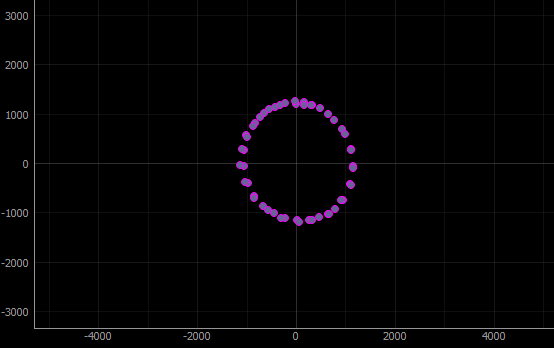
\includegraphics[width=0.6\linewidth]{rys/ScanBot-11-2d-set-theta-then-sigma-and-done.PNG}
	\caption{Chmura punktów po dokonaniu korekcji obu typów zniekształceń}
	\label{fig:2d-mag-soft-corr-applied}
\end{figure}

Finalna wersja aplikacji korzysta z dwóch osi magnetometru. W celu kalibracji należy skorzystać z zakładki \emph{magnetometer calibration} głównego okna aplikacji sterującej. Rysunek \ref{fig:main-app-mag-section-bottom} przedstawia najważniejsze elementy tej zakładki, wykorzystywane podczas półautomatycznego procesu kalibracji.

\begin{figure}[ht]
	\centering
		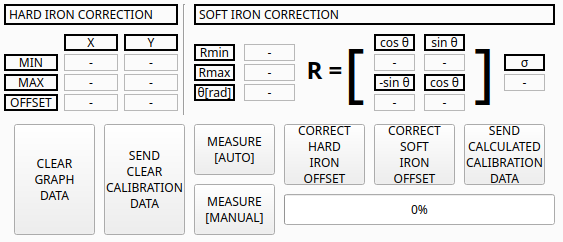
\includegraphics[width=1\linewidth]{rys/main-app-view-magnetom-bottom.png}
	\caption{Najważniejsze elementy sekcji kalibracji}
	\label{fig:main-app-mag-section-bottom}
\end{figure}

Aby dokonać kalibracji, robot powinien być połączony z aplikacją sterującą. Dalej procedura przebiega jak następuje:

\begin{enumerate}
    \item Należy przejśćdo zakładki \emph{magnetometer calibration}
    \item Jeżeli na wykresie znajdują się poprzednie pomiary, należy kliknąć przycisk \emph{CLEAR GRAPH DATA} aby je usunąć
    \item Należy wyzerować dane kalibracyjne znajdujące się w pamięci EEPROM robota. Służy do tego przycisk \emph{SEND CLEAR CALIBRATION DATA}
    \item Na tym etapie istnieją dwie możliwości przeprowadzenia pomiaru - za pomocą przycisku \emph{MEASURE [AUTO]} platforma samodzielnie, krokowo, wykona obrót wokół własnej osi i zbierze serię pomiarów z magnetometru; za pomocą przycisku \emph{MEASURE [MANUAL]} dokona jedynie pomiarów, w tym czasie należy robota obracać ręcznie. Postęp pomiarów wizualizowany jest na pasku postępu w prawym dolnym rogu. Na wykresie pojawią się zebrane pomiary. W sekcji oznaczonej \emph{HARD IRON CORRECTION} pojawiać się będą uzyskane dane dotyczące korekcji pierwszego z omawianych wcześniej zaburzeń - wartości minimalne i maksymalne dla każdej z osi oraz wartość przesunięcia (\emph{OFFSET}). W sekcji \emph{SOFT IRON CORRECTION} pojawiać się będą cyklicznie przeliczane wartości dotyczące korekcji zaburzeń \emph{soft iron} - m.in. parametry $\theta$ $\sigma$ i wartości macierzy $R$.
    \item Za pomocą przycisku \emph{CORRECT HARD IRON OFFSET} należy dokonać korekcji zaburzeń typu \emph{hard iron} na podstawie obliczonych wartości przesunięcia. Efekt natychmiastowo ukaże się na wykresie.
    \item Za pomocą przycisku \emph{CORRECT SOFT IRON OFFSET} należy dokonać korekcji zaburzeń typu \emph{soft iron}. Dane również brane są z obliczonych podczas procedury pomiaru. W tym momencie punkty na wykresie powinny być ułożone w okrąg. Jeżeli jest inaczej, oznacza to że w otoczeniu występują zaburzenia pola magnetycznego. Wtedy należy przemieścić robota w inne miejsce i powtórzyć wymienione czynności od nowa.
    \item Na koniec, aby wysłać dane kalibracyjne do robota, należy kliknąć przycisk \emph{SEND CALCULATED CALIBRATION DATA}. 
\end{enumerate}

Po dokonaniu procedury kalibracji pomiary dużo lepiej oddają rzeczywisty kierunek i zwrot platformy, jednak nawet podczas postoju platformy zwracana wartość azymutu nie pozostaje stała. Aby zniwelować to zjawisko konieczne jest zastosowanie filtru.

\subsection{Filtr Kalmana}
W układach sensorycznych robotów powszechnie wykorzytywany jest filtr Kalmana\cite{Kedzierski2016}. W tej sekcji wyjaśniona będzie zastosowana w projekcie, uproszczona implementacja takiego filtru.

\begin{listing}[ht]
\begin{minted}[fontsize=\footnotesize]{python}
def get_azimuth_kalman(self):
    q = 0.1
    estimate_err = 3
    measure_err = 3
    last_est = int(self.send("GET_AZIMUTH#"))

    for _ in range(20):
        measurement = int(self.send("GET_AZIMUTH#"))
        kalman_gain = estimate_err/(estimate_err + measure_err)
        current_est = last_est + kalman_gain*(measurement - last_est)
        estimate_err = (1 - kalman_gain)*estimate_err + abs(last_est-current_est)*q
        last_est = current_est
        ... (pominięto)
        
    current_est = int(current_est)
    self.azimuth = current_est
    self.publish_ros_odometry()
    return self.azimuth
\end{minted}
\caption{Implementacja filtru Kalmana w języku Python}
\label{lst:kalman}
\end{listing}

Ze względu na ograniczone zasoby mikrokontrolera, filtracja odbywa się po stronie aplikacji sterującej. Pomiar dokonywany jest podczas gdy platforma stoi nieruchomo, stąd wiadomo że estymowana wartość jest stała. Na początku potrzebne będzie kilka odgórnie ustalonych parametrów. Wartości \emph{estimate\_err} i \emph{measure\_err} odpowiadają kolejno wariancji estymatora i wariancji mierzonej wartości (normalnie wyznaczone na podstawie dokładności pomiaru przyrządu), jednak nie muszą one być ustalone na podstawie rzeczywistych parametrów urządzenia. Ich wartości będą wpływać na działanie filtru - to czy dane będą bardziej "wygładzane", czy bardziej zależne od ostatniego pomiaru. W tym wypadku zostały wyznaczone eksperymentalnie. Parametr \emph{q} nie był konieczny, służy on regulacji zwiększenia wariancji estymaty w przypadku gdy estymowana wartość jest zmienna w czasie. Został on również dobrany eksperymentalnie. Chociaż ma mały wpływ na pomiary statyczne - jest zaimplementowany na potrzeby przyszłego rozwoju projektu.

Kolejną rzeczą która jest potrzebna jest aktualna wartość ostatniej estymacji \emph{last\_estimate}. Przy odpowiednio długim pomiarze tę wartość można ustawić na dowolną, jednak aby wartość estymatora szybciej zbiegała do estymowanej wstępnie zostaje ustawiona na zmierzoną wartość.

Mając wszystkie parametry można przystąpić do uruchomienia filtru. Przebiega on w 20 iteracjach - wartość ta została dobrana arbitralnie w celu ewentualnej późniejszej korekcji. Nie mogła być zbyt duża, aby mikrokontroler był w stanie ukończyć operację pomiaru w rozsądnym czasie. W każdej z iteracji zachodzą dwie fazy - predykcji i korekcji.
\\

Faza predykcji polega na wyznaczeniu wartości oczekiwanej apriori $\hat{x}(t+1)^-$ i odchylenia standardowego apriori $\sigma^2(t+1)^-$ dla czasu $t+1$ na podstawie analogicznych wartości aposteriori dla czasu $t$, tj.  $\hat{x}(t)^+$ i $\sigma^2(t)^+$. W tym wypadku z założenia wartość mierzona jest stała, dlatego przyjmuje się, że:

\begin{equation}
\begin{aligned}
    \hat{x}(t+1)^- = \hat{x}(t)^+ \\
    \sigma^2(t+1)^- = \sigma^2(t)^+    
\end{aligned}
\label{eq:x-apriori-aposteriori}
\end{equation}

Kod programu korzysta ze zmiennych \emph{est\_error} i \emph{current\_est}. Wartości apriori i aposteriori nie muszą być przechowywane jednocześnie w pamięci - wystarczy nadpisywać stare zmienne. Tutaj oznaczałoby to sformułowanie konstrukcji \emph{est\_error}=\emph{est\_error} i \emph{current\_est}=\emph{current\_est} co nie jest potrzebne i dlatego zostało pominięte.
\\

Faza korekcji odbywa się w pętli. Najpierw dokonywany jest pomiar z sensora (\emph{measurement}). Następnie obliczane jest wzmocnienie Kalmana (\emph{kalman\_gain}), czyli parametr wpływający na to jakie znaczenie nowy pomiar ma dla wartości estymatora oraz jego wariancji. Później, z jego wykorzystaniem obliczana jest nowa wartość estymatora (\emph{current\_est}). W kolejnej linijce aktualizowana jest wartość jego wariancji (\emph{estimate\_err}). Aktualnie wraz z każdym nowym przejściem pętli zbiega ona do niezerowej wartości, zależnej od parametru q. Gdyby ten parametr nie zaistniał, z każdą iteracją jej wartość zbiegałaby do zera. Na koniec wartość (\emph{current\_est}) kopiowana jest do (\emph{last\_est}). Dzieje się to, ponieważ aktualizacja (\emph{estimate\_err}) potrzebuje przy obliczeniach wartości aktualnej oraz poprzedniej estymatora.

Po dwudziestokrotnym przejściu, wartość oczekiwana estymatora konwertowana jest na liczbę całkowitą, i zapisywanam, dane o azymucie są publikowane na odpowiednim temacie i wartość jest zwracana przez funkcję.

\subsection{Poprawa jakości odometrii}
\label{sec:umbmark}
Ze względu na brak możliwości skonstruowania idealnego obiektu rzeczywisty ruch platformy nie pokrywa się z zamierzonym. Oś obrotu kół nigdy nie osiągnie wymiarów idealnie równych z projektem, podobnie same koła będą miały inne i różne od siebie średnice (oczywiście, z pewnym przybliżeniem mówi się że są one ``równe``). Dodatkowo na nieidealny tor ruchu wpływa chropowatość powierzchni, drgania styków enkoderów i wiele innych czynników. Istnieje metoda która pozwala skorygować część z wymienionych czynników.
\\

Wykorzystana zostanie metoda korekcji opisana w pracy \emph{Correction of Systematic Odometry Errors in Mobile Robots}\cite{Borenstein1995}. Korzysta ona z metody wyznaczania błędu przejazdu trasy zwanej \emph{UMBmark} (od ang. \emph{University of Michigan Benchmark}). Polega ona na zbadaniu przesunięcia pozycji końcowej robota względem pozycji początkowej po pokonaniu wyznaczonej, kwadratowej ścieżki. Na rysunku \ref{fig:umbenchmark-path} przedstawiono przykładowy przejazd w kierunku przeciwnym do ruchu wskazówek zegara.

\begin{figure}[ht]
	\centering
		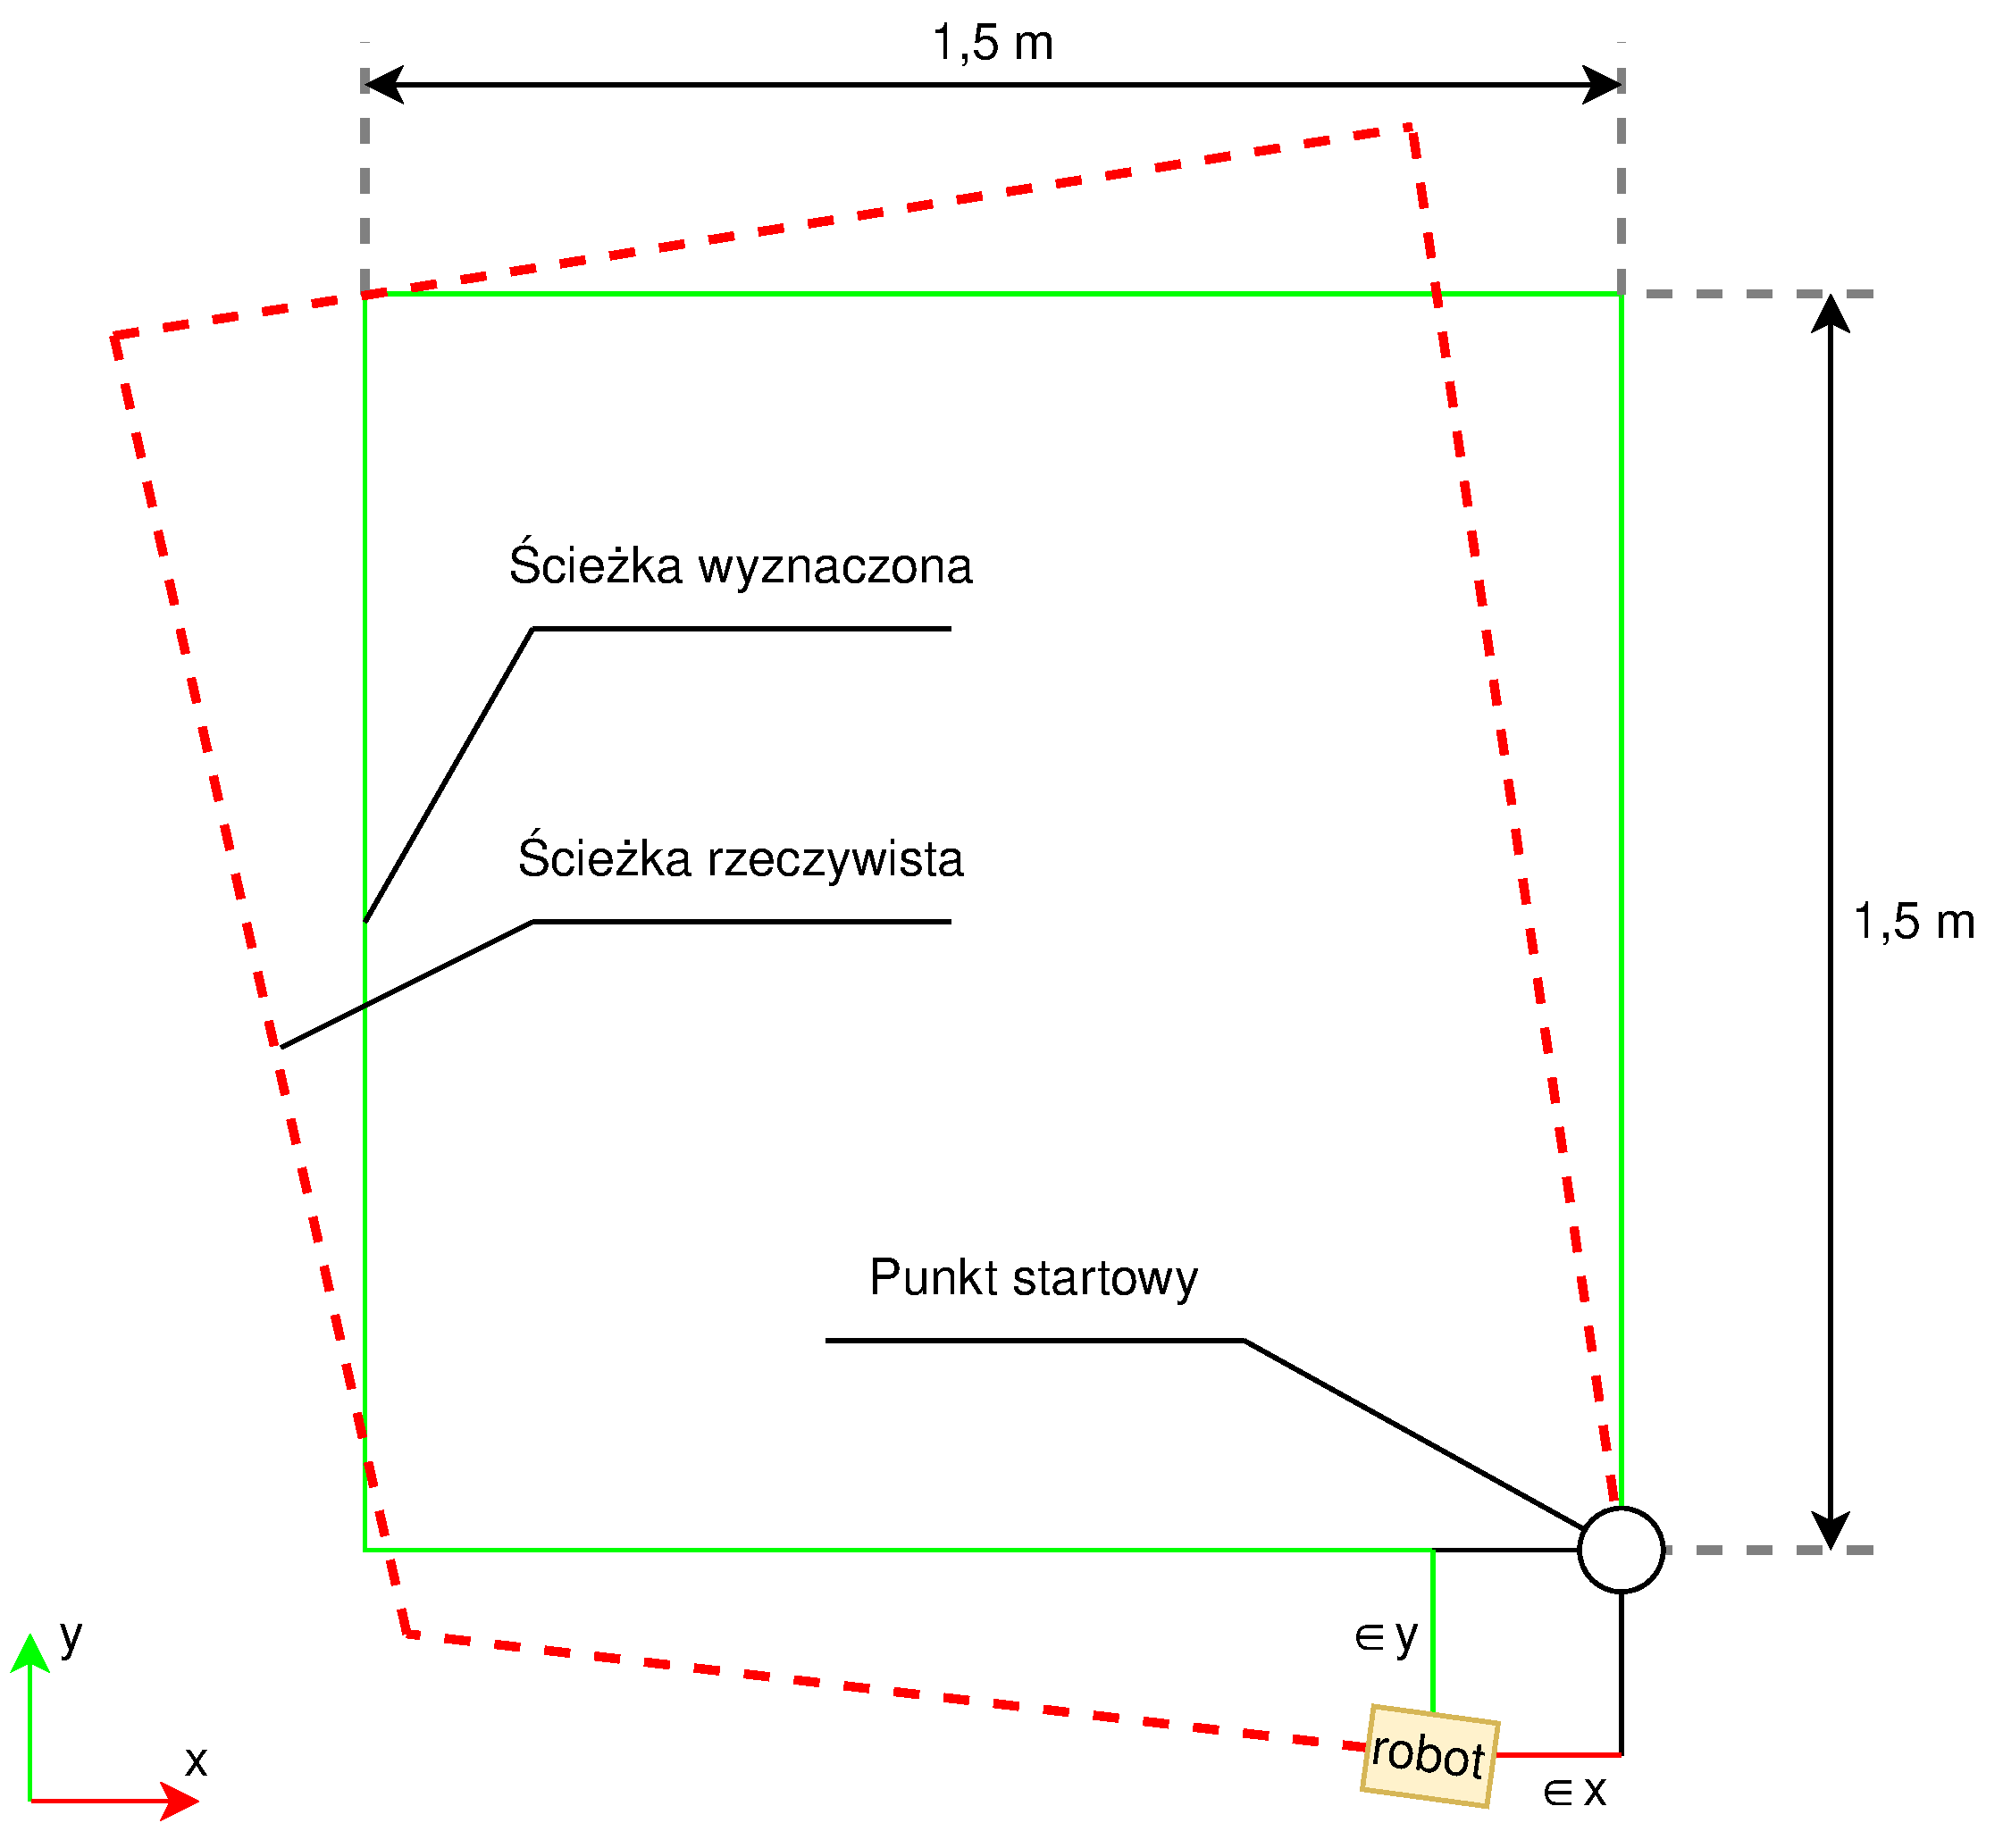
\includegraphics[width=0.8\linewidth]{rys/umbenchmark-path.pdf}
	\caption{Trasa przejazdu robota według \emph{UMBmark}}
	\label{fig:umbenchmark-path}
\end{figure}

Metoda \emph{UMBmark} polega na pięciokrotnym pomiarze błędów $\in{x}$ oraz $\in{y}$ po przejazdach zgodnie i przeciwnie do ruchu wskazówek zegara. Różne kierunki przejazdu pomogą zniwelować wpływ błędów niesystematycznych na tor jazdy platformy. Rozmiar kwadratowej ścieżki według dokumentu powinien wynosić $4\times4$ metry ($L=4m$), jednak ze względu na ograniczoną przestrzeń autor zmniejszył obszar do rozmiaru $1,5\times1,5$ metra. Zdjęcia środowiska testowego przedstawiono na rys. \ref{fig:umbenchmark-photo-path} i  \ref{fig:umbenchmark-photo-finish}. Do pomiarów użyto taśmy mierniczej zwijanej o dokładności ±1 mm jednak ze względów praktycznych w pomiarach uwzględniono wartości zaokrąglone do pełnych centymetrów. Wyniki przedstawiono w tabeli \ref{tab:umbmark}.

\begin{figure}[ht]
	\centering
		\includegraphics[width=0.6\linewidth]{rys/UMBenchmark-1.jpg}
	\caption{Wyznaczona ścieżka przejazdu robota}
    \label{fig:umbenchmark-photo-path}
\end{figure}

\begin{figure}[ht]
	\centering
		\includegraphics[width=0.6\linewidth]{rys/UMBenchmark-2.jpg}
	\caption{Punkt startowy i przesunięcie}
    \label{fig:umbenchmark-photo-finish}
\end{figure}


\begin{table}[H]
    \caption{Wyniki pomiarów \emph{UMBmark}}
     \label{tab:umbmark}
    \centering
    \begin{tabular}{ |p{0.05\linewidth}|p{0.15\linewidth}|p{0.15\linewidth}|p{0.15\linewidth}|p{0.15\linewidth}| } \hline
    N. p. & \multicolumn{2}{p{0.15\linewidth}|}{Kierunek: $\circlearrowleft$} & \multicolumn{2}{p{0.15\linewidth}|}{Kierunek: $\circlearrowright$} \\ \hline
    - & $\in{x}$ & $\in{y}$ & $\in{x}$ & $\in{y}$ \\ \hline \hline
    1 & -28 & 5 & 62 & 28 \\ \hline
    2 & -33 & 15 & 54 & 32 \\ \hline
    3 & -2 & 4 & -45 & 9 \\ \hline
    4 & -5 & -21 & -55 & -19 \\ \hline
    5 & 13 & -12 & -31 & 27 \\ \hline
\end{tabular}
\end{table}

Mając do dyspozycji wartości potrzebnych pomiarów można przystąpić do obliczeń. Najpierw dla każdego kierunku należy wyznaczyć środek ciężkości, czyli uśrednić wartości współrzędnych $x$ i $y$, gdzie przykładowo dolny indeks $x_{cgcw}$ oznacza wartość współrzędnej $x$ środka ciężkości dla przejazdów zgodnych z ruchem wskazówek zegara (ang. \emph{cg - center of gravity}, \emph{cw - clockwise}). Analogicznie dla kierunku przeciwnego to będzie $x_{csccw}$. I tak:

\begin{equation}
\begin{aligned}
    x_{cgccw} = \frac{1}{n}\sum_{i=1}^{n} (\in{x_{i,ccw}}) = \frac{-28-33-2-5+13}{5} = -11 \\[5pt]
    y_{cgccw} = \frac{1}{n}\sum_{i=1}^{n} (\in{y_{i,ccw}}) = \frac{5+15+4-21-12}{5} = -1,8 \\[5pt]
    x_{cgcw} = \frac{1}{n}\sum_{i=1}^{n} (\in{x_{i,cw}}) = \frac{62+54-45-55-31}{5} = -3 \\[5pt]
    y_{cgcw} = \frac{1}{n}\sum_{i=1}^{n} (\in{y_{i,cw}}) = \frac{28+32+9-19+27}{5} = 15,4
\end{aligned}
\end{equation}

W kolejnym kroku zostaną obliczone współczynniki $\alpha$ oraz $\beta$:

\begin{equation}
\begin{aligned}
    \alpha = \frac{x_cgcw + x_cgccw}{-4L} = \frac{-3 - 11}{-4 \times 1,5} = 2,33^{\circ} \\[5pt] 
    \beta = \frac{x_cgcw - x_cgccw}{-4L} = \frac{-3 + 11}{-4 \times 1,5} = -1,33^{\circ}
\end{aligned}
\end{equation}

Z pomocą współczynników $\alpha$ i $\beta$ obliczane są błędy wylistowane poniżej. Tu należy zaznaczyć, że korekta dotyczy parametrów długości osi $b$ i średnicy kół $D$ schematu zastępczego robota przedstawionego wcześniej w niniejszym dokumencie na rysunku \ref{fig:odom-axis-simplified}.

\begin{itemize}
    \item Błąd $E_{d}$ będący stosunkiem średnicy koła prawego do koła lewego
    \item Błąd $E_{b}$ będący stosunkiem rzeczywistej długości osi do długości nominalnej
\end{itemize}

\begin{figure}[ht]
	\centering
		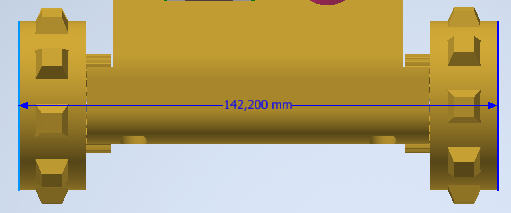
\includegraphics[width=0.6\linewidth]{rys/axis-b-param.PNG}
	\caption{Długość nominalna osi robota}
    \label{fig:nominal-axis-width}
\end{figure}


Obliczanie współczynników $R$, $E_{d}$ i $E_{b}$ ukazano poniżej. Przydatny będzie tutaj parametr $b$ oznaczający rozpiętość osi zastępczej pojazdu. Jest ona równa osiom rzeczywistym i wynosi 14,22 centymetrów, co uwidoczniono na rysunku \ref{fig:nominal-axis-width}.

\begin{equation}
\begin{aligned}
    R = \frac{L : 2}{sin(\beta : 2)} = \frac{1,5 : 2}{sin(-1,33 : 2)} = -0,01 \\[5pt]
    E_{d} = \frac{R + (b : 2)}{R - (b : 2)} = \frac{-0,01 + (14,22 : 2)}{-0,01 - (14,22 : 2)} = -0.997 \\[5pt]
    E_{b} = \frac{90^{\circ}}{90^{\circ} - \alpha} = \frac{90^{\circ}}{90^{\circ} - 2,33^{\circ}} = 1,03
\end{aligned}
\end{equation}


Parametr $R$ posłużył jedynie obliczeniu pozostałych dwóch. Współczynnik $E_{d}$ odnosi się do korekcji błędów typu b opisanych w pracy Borenstein'a (zakrzywiony tor jazdy) i jest równy stosunkowi średnic przeciwległych kół (modelu zastępczego) pojazdu. Specjalnie, w odróżnieniu do innych wartości został zaokrąglony do trzeciego miejsca po przecinku - w innym wypadku wynosiłby 1. Z tego samego powodu można uznać, że korekcja uwzględniająca ten parametr nie jest konieczna - robot jeździ wystarczająco "prosto" a ewentualne zakrzywienie toru jazdy wynika z czynników niesystematycznych (zmiany powierzchni, nierówności).

Jeżeli chodzi o $E_{b}$ odnosi się on do korekcji błędów typu a - zbyt dużych lub za małych zakrętów wykonywanych w miejscu przez robota. Taki błąd wynika z różnicy między nominalnym a rzeczywistym rozstawem kół pojazdu. Stosunek tych wartości opisuje wartość tegoż współczynnika wynosząca 1,03. Oznacza to że robot podczas obrotu zachowuje się tak, jakby jego oś była dłuższa o 3\% niż przewidziano w projekcie. Mając na uwadzę czynnik jakim jest poślizg gąsienic oraz zgrubny charakter aproksymacji jego modelu, autor na podstawie pewnych intuicji i poprzednich doświadczeń był w stanie stwierdzić że taki błąd jest pomijalny. Dodatkowo, ze względu na eksperymentalny charakter implementacji zakrętu w niniejszym projekcie zastosowanie takiej korekcji byłoby bardziej skomplikowane, ponieważ długość osi nie jest nigdzie zdefiniowana.

\section{Skan otoczenia i budowa mapy}
\label{sec:scan}
Samo zebranie pomiarów i przedstawienie ich w formie czytelnej dla człowieka nie jest trudne w realizacji. Pozyskane dane można przedstawić na wykresie, punkty połączyć prostymi liniami. Problem zaczyna się z agregacją wielu pomiarów, i na tym będzie koncentrował się ten rozdział.

Mając do dyspozycji dane z sensora \emph{LIDAR} oraz enkoderów i magnetometru, można rozpocząć proces skanowania. Pierwsze podejście oparte było o skan manualny, bez zliczania ścieżki - jedynie obrót był uwzględniony a dane ze skanera obracane o zczytany z sensora azymut. Robot został ustawiony w początkowej pozycji, uruchomiono procedurę skanowania za pomocą funkcji \emph{SCAN}, następnie z racji że skan zachodzi w zakresie kątów $\langle0^{\circ},180^{\circ}\rangle$, obrócony o $180^{\circ}$ (funkcja \emph{ROTATE}) po czym ponownie wykonano skanowanie. Efekt przedstawia rysunek\ref{fig:first-scan}. Jak widać, ściany pokoju (górna i dolna część rysunku) nie są równoległe. W tym momencie okazało się, że konieczna będzie kalibracja magnetometru, omówiona w rozdziale \ref{sec:odometry}. Po dokonaniu procedury kalibracji czynności powtórzono, rezultat ukazano na rysunku \ref{fig:first-magnetom-calibrated-scan}. Na dalej przedstawianych rysunkach skany mogą wyglądać nieco inaczej, głównie przez zamknięte lub otwarte drzwi pokoju - widoczne jest to na ostatnich dwóch wspomnianych rysunkach jako najdłuższe z promieni - w tym wypadku drzwi były otwarte a pomiar uwzględniał fragment przedpokoju autora. Skany przedstawiane są w zakładce \emph{map} okna głównego aplikacji sterującej.

\begin{figure}[ht]
	\centering
		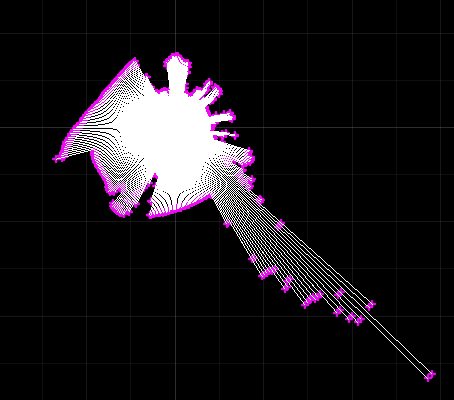
\includegraphics[width=0.6\linewidth]{rys/ScanBot-01-room-map-nocalibration.png}
	\caption{Pierwszy skan pokoju}
	\label{fig:first-scan}
\end{figure}

\begin{figure}[ht]
	\centering
		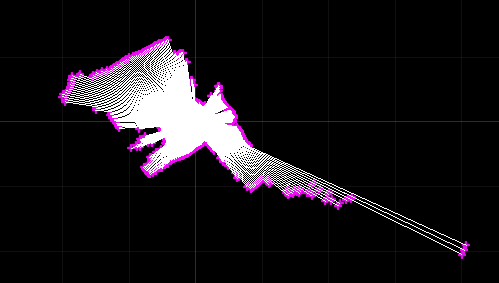
\includegraphics[width=0.6\linewidth]{rys/ScanBot-02-room-map-calibrated.png}
	\caption{Skan pokoju po zastosowaniu kalibracji magnetometru}
	\label{fig:first-magnetom-calibrated-scan}
\end{figure}

W opisanych krokach dwa przeprowadzane pomiary były od siebie niezależne - mierzyły odległość od innych obiektów. Kolejnym krokiem było wykonanie kilku pomiarów częściowo nakładających się na siebie, co przedstawiają rysunki \ref{fig:overlapping-1}, \ref{fig:overlapping-2}, \ref{fig:overlapping-3} i \ref{fig:overlapping-4}. Szczególnie należy zwrócić uwagę na ostatni z nich - wyraźnie widać że ostatni skan absolutnie nie pokrywa się z poprzednimi. Najwyraźniej sama informacja o aktualnej rotacji robota nie jest wystarczająca aby dokładnie umieścić punkty na płaszczyźnie. 

\begin{figure}[ht]
	\centering
		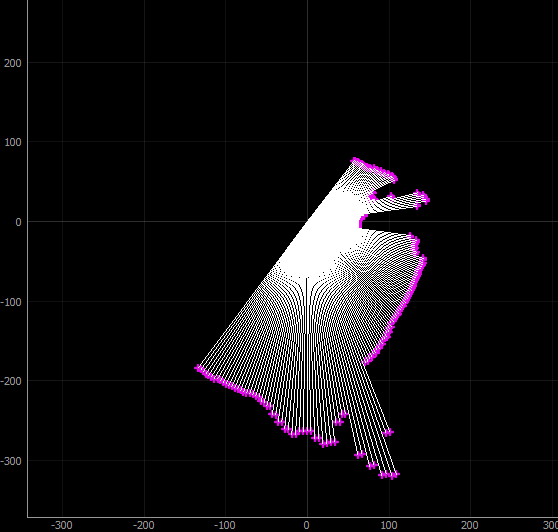
\includegraphics[width=0.5\linewidth]{rys/ScanBot-12-calibrated-room-map1.PNG}
	\caption{Skan pierwszy}
	\label{fig:overlapping-1}
\end{figure}

\begin{figure}[ht]
	\centering
		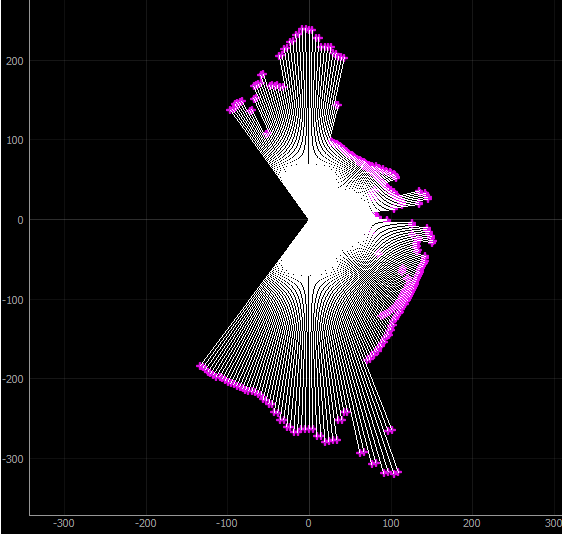
\includegraphics[width=0.5\linewidth]{rys/ScanBot-12-calibrated-room-map2.PNG}
	\caption{Skan drugi}
	\label{fig:overlapping-2}
\end{figure}

\begin{figure}[ht]
	\centering
		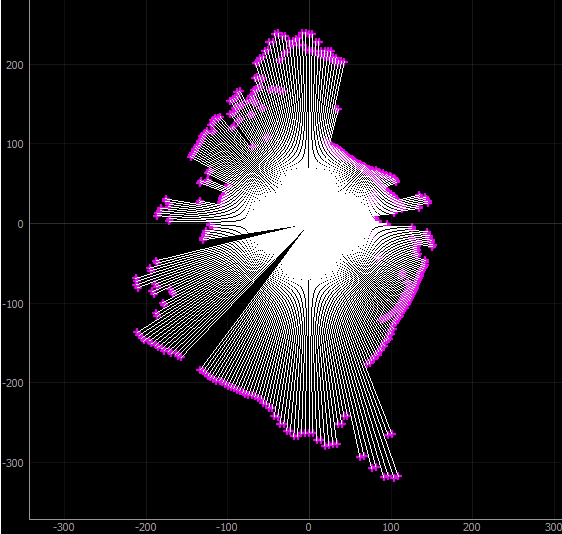
\includegraphics[width=0.5\linewidth]{rys/ScanBot-12-calibrated-room-map3.PNG}
	\caption{Skan trzeci}
	\label{fig:overlapping-3}
\end{figure}

\begin{figure}[ht]
	\centering
		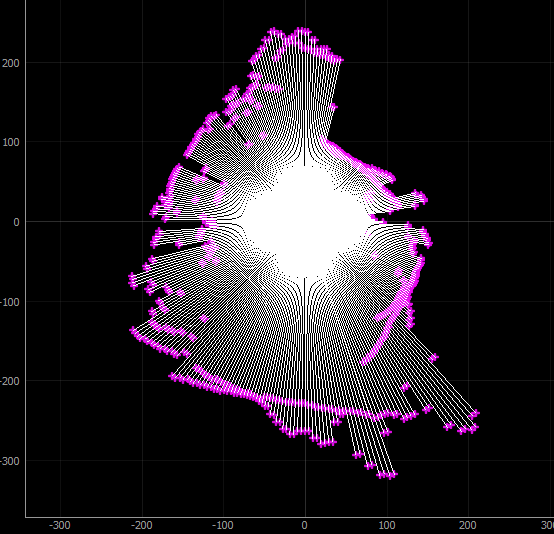
\includegraphics[width=0.5\linewidth]{rys/ScanBot-12-calibrated-room-map4.PNG}
	\caption{Skan czwarty}
	\label{fig:overlapping-4}
\end{figure}

W celu korekcji rzutowania punktów na płaszczyznę, pierwotnie stosowany był opracowany przez autora prosty, naiwny algorytm korygujący rotację. Jego działanie można opisać w kilku krokach. (Algorytm \ref{pcode:rotation-correction}).

\begin{algorithm}[ht]
\SetAlgoLined
\SetAlgorithmName{Algorytm}{}\\

// Pierwszy skan nie jest korygowany, ponieważ nie ma innych punktów na mapie \\ 
kąty, odległości = wykonaj\_skan() \\
azymut = zmierz\_azymut() \\
\For{i = 0, ..., 180}{
    kąty[i] = kąty[i] + azymut \\ 
}
\EndFor\\[10pt]

nanieś\_na\_wykres(kąty, odległości) \\[10pt]

\While{program\_jest\_uruchomiony}{
    kąty, odległości = wykonaj\_skan() \\
    azymut = zmierz\_azymut() \\
    \For{i = 0, ..., 180}{
        kąty[i] += azymut \\ 
    }
    \EndFor\\[10pt]
    
    // Słownik przechowujący wartości \emph{score} \\ 
    // dla poszczególnych par klucz:wartość ( kąt\_korekcji:score) \\ 
    score = \{\} \\ [10pt]
    
    \For{i = -10, ..., 10}{
        kąty\_temp[i] = kąty[i] + i  \\
        score[i] = oblicz\_score(kąty\_temp, odległości, punkty\_na\_mapie) \\
    }
    \EndFor\\[10pt]
    
    \eIf{max(score.wartości()) > 2500}{
        kąt\_korekcji = max(score.wartości()).klucz() \\ 
        \For{i = 0, ..., 180}{
            kąty[i] += kąt\_korekcji  \\
        }
        \EndFor\\
        nanieś\_na\_wykres(kąty, odległości) \\
        azymut\_robota += kąt\_korekcji
    }{
        // Nie stosuj korekcji \\
        nanieś\_na\_wykres(kąty, odległości) \\
    }
}
\EndWhile\\[10pt]

\caption{Korekcja rotacji zmierzonych punktów}
\label{pcode:rotation-correction}
\end{algorithm}

%%%%%%%%%%%%%%%%%%%%%%%%%%%%%%%%%%%%%%%%%%%%%%%%%%%%%%%%%%%%%%%%%%%%%%%%%%%%%%%%%%%%%%%%%%%%%%%%%%
%%%%%%%%%%%%%%%%%%%%%%%%%%%%%%%%%%%%%%%%%%%%%%%%%%%%%%%%%%%%%%%%%%%%%%%%%%%%%%%%%%%%%%%%%%%%%%%%%%
% \begin{enumerate}
%     \item Na początku należy przeprowadzić pierwszy skan i zmierzyć azymut w którym skierowany jest robot.
%     \item Następnie pomiary ze skanu (odległości w cm dla każdego z całkowitych wartości kątów w zakresie $\langle0^{\circ}, 180^{\circ}\rangle$) należy nanieść na wykres, uwzględniając rotację robota (dodając zmierzony azymut do wartości kątów przypisanych do każdego z pomiarów skanu).
%     \item Potem przeprowadzany jest kolejny skan i pomiar azymutu.
%     \item Do każdego z kątów pomiaru skanu dodawany jest azymut.
%     \item W pętli, dla każdej z wartości $i$, gdzie $i={-10,-9,...,9,10}, i \in \mathbb{Z}$ do każdego z kątów dodawana jest wartość $i$ oraz sprawdzany i zapisywany jest parametr \emph{score} w sposób opisany w dalszej części dokumentu.
%     \item Sprawdzane jest dla jakiego $i$ wartość parametru \emph{score} była największa. 
%     \item Wyszukana wartość $i$ jest ostatecznie dodawana do wartości każdego z kątów pomiaru razem ze zmierzonym azymutem. Ta sama wartość jest dodawana do azymutu w którym skierowany jest robot - w ten sposób następuje jego korekcja. Kolejny pomiar i korekcja następuje od punktu 3 niniejszej listy.
% \end{enumerate}
%%%%%%%%%%%%%%%%%%%%%%%%%%%%%%%%%%%%%%%%%%%%%%%%%%%%%%%%%%%%%%%%%%%%%%%%%%%%%%%%%%%%%%%%%%%%%%%%%%
%%%%%%%%%%%%%%%%%%%%%%%%%%%%%%%%%%%%%%%%%%%%%%%%%%%%%%%%%%%%%%%%%%%%%%%%%%%%%%%%%%%%%%%%%%%%%%%%%%

Listing \ref{lst:score-angle-correction} przedstawia fragment kodu przeprowadzający obliczanie współczynnika \emph{score}. Tutaj należy zaznaczyć, że ze względu na liczne zmiany w projekcie ten fragment nie zachował się w finalnej wersji kodu, można go natomiast podejrzeć na rezpozytorium w pliku \emph{src-pc/main.py} na gałęzi \emph{master} pod \emph{commit id} wynoszącym aba2c1510f1a661e6365f9cd4ca7dc782f013593.

\begin{listing}[H]
\begin{minted}[fontsize=\footnotesize]{python}

def calc_xy_overlap_score(self, points1, points2):
    score = 0
    for point in points1:
        distance = self.find_xy_closest_point_distance(
            [point[0], point[1]], points2)
        # important! this way we're avoiding very high 1/distance value
        distance = int(distance)
        if distance == 0:
            score += 100
        elif distance >= 100:
            pass
        else:
            score += int((1/distance)*100)
    return score
\end{minted}
\caption{Obliczanie współczynnika \emph{score} i korekcja kąta w celu dopasowania pomiaru do mapy}
\label{lst:score-angle-correction}
\end{listing}

Współczynnik \emph{score} obliczany jest na podstawie podobieństwa między pozycją punktów z najnowszego skanu względem tego, co już znajduje się na mapie. Aby móc skorzystać z powyższej funkcji poszczególne pomiary dla skanu są przeliczane z postaci biegunowej na kartezjańską. Następnie jest ona uruchamiana, a do parametrów \emph{points1} i \emph{points2} kolejno przekazywane są listy punktów nowego skanu i punktów znajdujących się na mapie. W dalszej kolejności dla każdego z punktów skanu wykonywana jest operacja znalezienia najbliższego punktu na mapie i obliczenia odległości między nimi. Jeżeli punkty idealnie się pokrywają, do \emph{score} dodawana jest wartość 100. Jeżeli ta odległość wynosi więcej lub równo 100 centymetrów, nie dodawana jest żadna wartość. W zakresie $(1,100)$ do współczynnika jest dodawana wartość równa $\frac{1}{odległość}*100$, zaokrąglona do najbliższej liczby całkowitej. 

\begin{listing}[H]
\begin{minted}[fontsize=\footnotesize]{c++}

if score > 2500:
    print(
        f"adjusted plot and robot rotation by {best_rotation} degrees.")
    rotated_data = self.rotate_points(filtered_data, best_rotation)
    self.robot.update_azimuth(self.robot.azimuth + best_rotation)
else:
    rotated_data = filtered_data
\end{minted}
\caption{Decyzja o zastosowaniu korekty}
\label{lst:score-threshold}
\end{listing}

Doświadczalnie został dobrany próg wartości \emph{score} równy 2500. Jeśli współczynnik dla najlepszej korekty kąta wynosi więcej niż próg, korekta zostanie zaakceptowana - azymut robota zostanie poprawiony, skan również będzie skorygowany i rzutowany na mapę. Obrazuje to listing \ref{lst:score-threshold}.

\begin{figure}[ht]
	\centering
		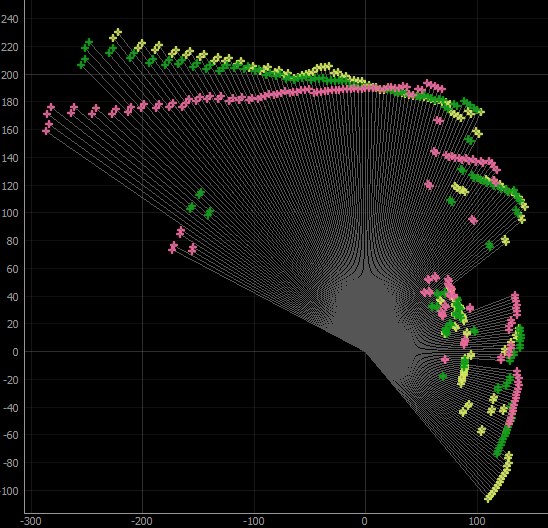
\includegraphics[width=0.6\linewidth]{rys/ScanBot-13-angular-alignment-1yellow-2pink-3correctedgreen.PNG}
	\caption{Zobrazowana zasada działania korekcji kąta przy użyciu współczynnika \emph{score}}
	\label{fig:score-alignment-rule}
\end{figure}

Na rysunku \ref{fig:score-alignment-rule} przedstawiono działanie algorytmu korekcji kąta. Drugi ze skanów (punkty oznaczone kolorem żółtym) jest korygowany względem danych znajdujących się na mapie pochodzących ze skanu pierwszego (kolor różowy). Widoczne jest spore przesunięcie. Pomiar różowy dopasowywany był w zakresie  ±10°, osiągając maksymalną wartość\emph{score} przy -10°. Skorygowany pomiar został naniesiony na mapę z kolorem zielonym.

Ewaluacja tego algorytmu dla całego pokoju została ukazana na rysunkach \ref{fig:score-alignment-eval-1} i \ref{fig:score-alignment-eval-2}.

\begin{figure}[ht]
	\centering
		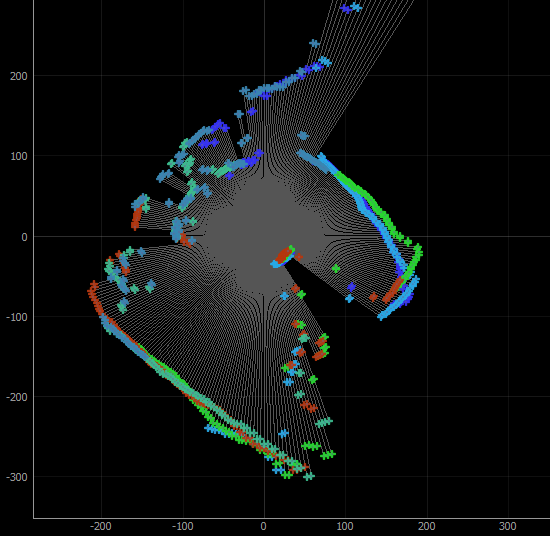
\includegraphics[width=0.6\linewidth]{rys/ScanBot-14-angular-alignment.PNG}
	\caption{Pięć skanów otoczenia nałożonych z pomocą korekcji korzystającej ze współczynnika \emph{score}}
	\label{fig:score-alignment-eval-1}
\end{figure}

\begin{figure}[ht]
	\centering
		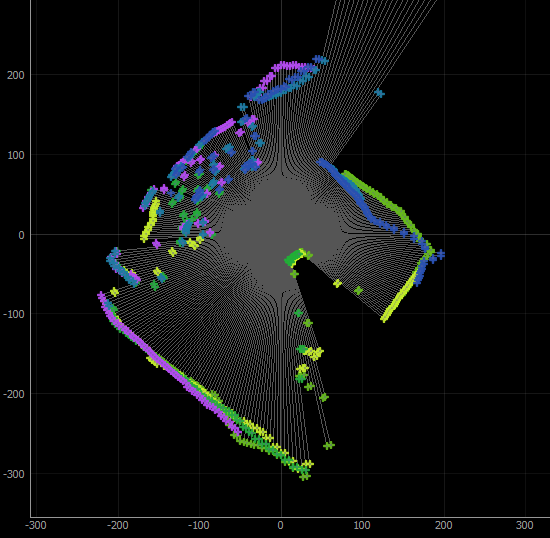
\includegraphics[width=0.6\linewidth]{rys/ScanBot-15-angular-alignment.PNG}
	\caption{Kolejne pięć skanów z korekcją kąta}
	\label{fig:score-alignment-eval-2}
\end{figure}

Pomimo iż algorytm działa i spełnia założone zadanie - problem \emph{SLAM} jest dużo bardziej złożony. Pierwotnie w planach autor planował wdrożenie podobnej korekcji dla translacji pojazdu oraz uśrednianie pozycji punktów na mapie. Jednak ze względu na dużą złożoność problemu i ograniczony czas autor zadecydował o skorzystaniu z istniejących rozwiązań. Pomocnym był tutaj zestaw narzędzi \emph{ROS}. Zawiera on wiele gotowych komponentów wykorzystywanych w robotyce, m. in. moduły adresujące problem \emph{SLAM}. Jednym z takich modułów jest \emph{slam\_gmapping} zawierający implementację algorytmu \emph{gmapping}\cite{Grisetti2005}\cite{gmapping-website}\cite{gmapping-ros}. Od tego momentu mapa sporządzana jest w środowisku \emph{ROS} i przedstawiana w programie \emph{RViz}. Finalna wersja aplikacji sterującej współpracuje ze środowiskiem publikując odpowiednie dane na wyznaczonych w tym celu tematach. Dokładniej obrazuje to schemat opisany w podrozdziale \ref{sec:pc-software}.

Kiedy całe środowisko zostało zestawione, przystąpiono do ręcznych testów jakości pracy platformy. Węzeł \emph{gmapping} uruchomiony został z parametrami domyślnymi. Już przy pierwszej ewaluacji (rysunek \ref{fig:mag-interference-first}) zauważono pewne nieprawidłowości. W tym momencie okazało się, że korzystanie z magnetometru przy odometrii nie było dobrym pomysłem. Pod podłogą prawdopodobnie w tym miejscu biegnie przewód elektryczny generując m. in. zmienne pole magnetyczne, zakłócając pracę magnetometru do takiego stopnia w którym odczytane dane są bezużyteczne i niemożliwe jest odtworzenie rzeczywistego pomiaru. Widoczne jest to w postaci bezładnie rozrzuconych punktów na górnej części rysunku, promieniujących od punktu w którym znajduje się robot.
\\

\begin{figure}[ht]
	\centering
	    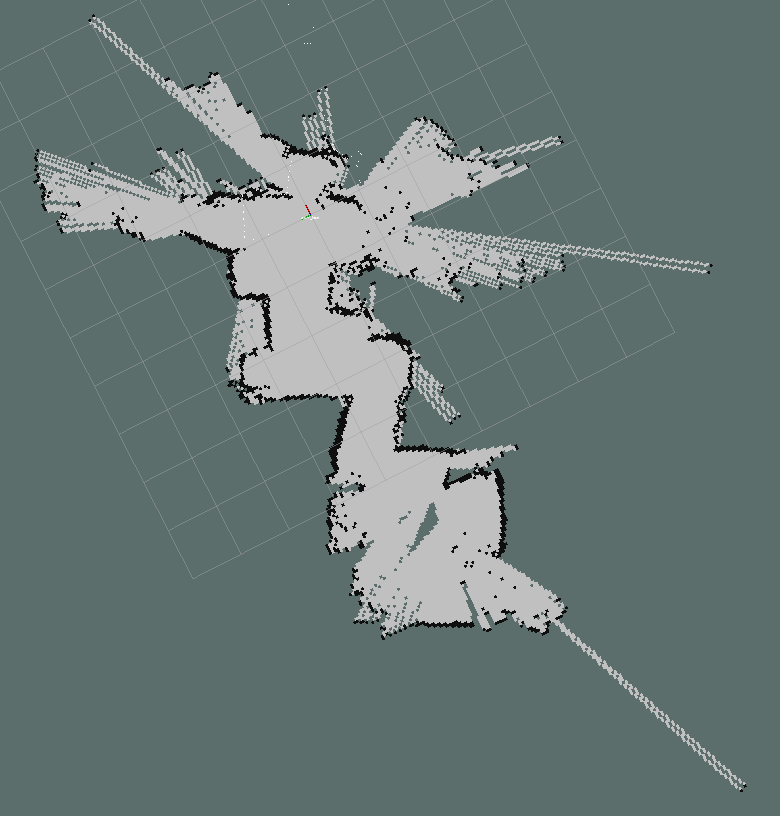
\includegraphics[width=0.6\linewidth]{rys/2020-11-04-170347_1920x1080_scrot.PNG}
	\caption{Mapa domu, uszkodzona na skutek interferencji magnetycznych}
	\label{fig:mag-interference-first}
\end{figure}

Aby zweryfikować przypuszczenia autor wykonał serię pomiarów za pomocą przycisku \emph{MEASURE [AUTO]} z zakładki \emph{magnetometer calibration}. To co zostało uwidocznione na rysunku \ref{fig:mag-interference-graph} z pewnością nie przypomina okręgu co potwierdza że w tym obszarze występują zakłócenia. Z tego powodu zmieniono sposób zliczania obrotu, co zostało opisane w rozdziale \ref{sec:odometry}.

\begin{figure}[H]
	\centering
		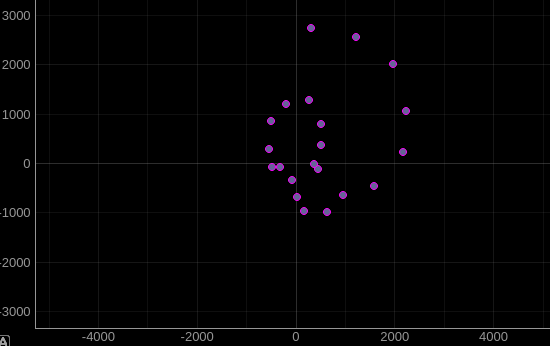
\includegraphics[width=0.6\linewidth]{rys/calibrated-mag-high-interference-broken-rotation.PNG}
	\caption{Seria pomiarów ze skalibrowanego magnetometru w obszarze silnych zakłóceń}
	\label{fig:mag-interference-graph}
\end{figure}

Niestety, wykorzystując mniej dokładną metodę zliczania algorytm \emph{gmapping} również traci na jakości działania. Pomiar jest odporny na zakłócenia magnetyczne ale występuje problem przy wjeździe robota do nowych pomieszczeń. Nie mając wielu punktów odniesienia, z dużym błędem rotacji nowe pokoje są wyraźnie obrócone względem stanu rzeczywistego co przedstawia rysunek \ref{fig:encoder-only-run-first} na którym zaznaczono również kolejność skanowania pomieszczeń (1 - pokój autora, 2 - przedpokój, 3 - kuchnia, 4 - drugi pokój). Wpływa to bardzo negatywnie na późniejsze pomiary - mimo wszelkich starań nie udało się ukończyć skanu wszystkich pokojów.
\\

\begin{figure}[H]
	\centering
		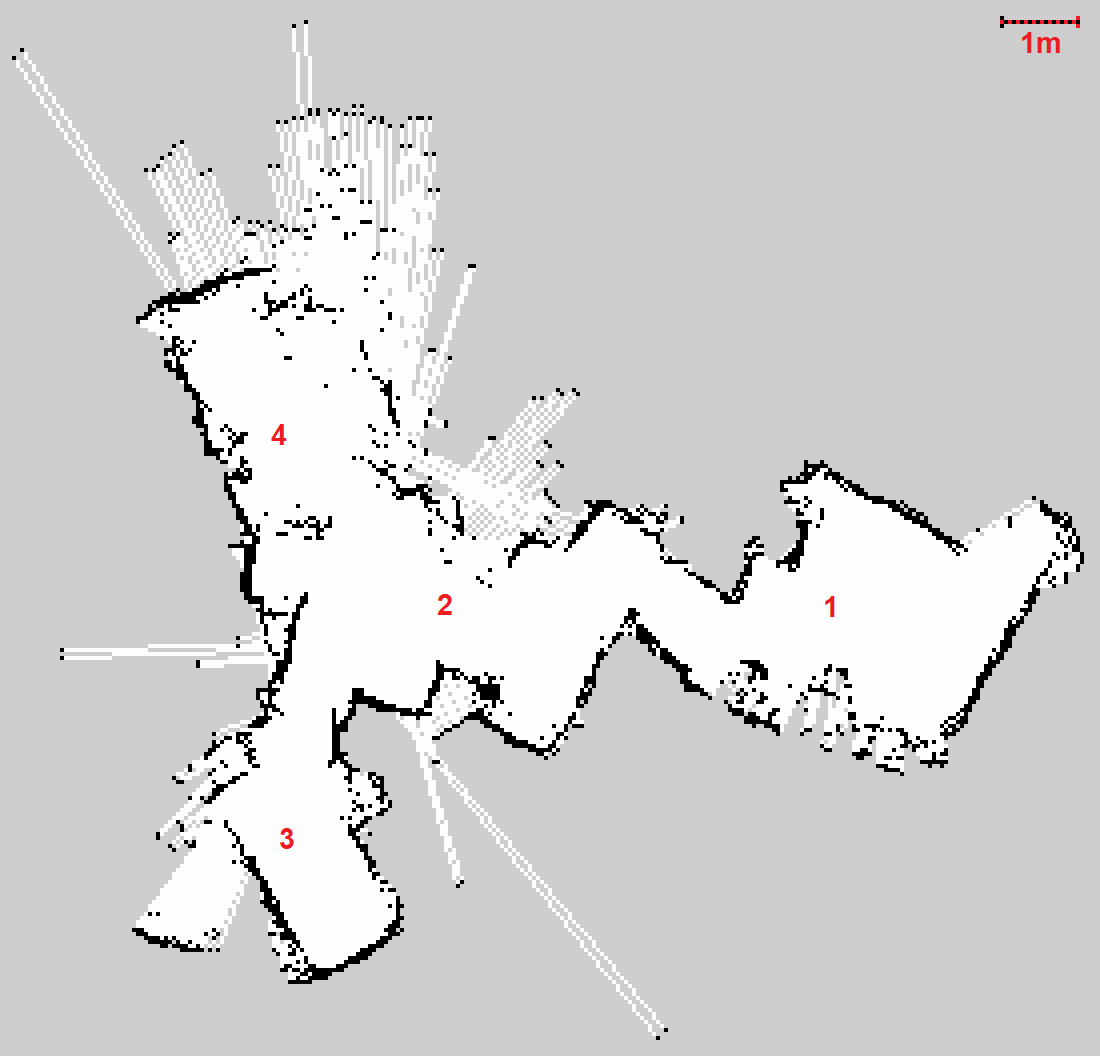
\includegraphics[width=0.8\linewidth]{rys/saved-map-2-encoder-only-cropped-upscaled-path-withscale.png}
	\caption{Mapa domu, obrót zliczany za pomocą enkoderów}
	\label{fig:encoder-only-run-first}
\end{figure}

Ze względu na długi czas ewaluacji skanu całego domu oraz szybko kumulujący się błąd, w dalszej części obszar został zawężony jedynie do pokoju autora. Zaimplementowany również został algorytm samodzielnej jazdy robota, opisany w podrozdziale \ref{sec:autonomous-drive}.

Wyniki dwóch przejść robota po pomieszczeniu autora z wykorzystaniem autorskiego algorytmu jazdy autonomicznej przedstawiono na rysunkach \ref{fig:final-scans}.


\begin{figure}[H]
	\centering
		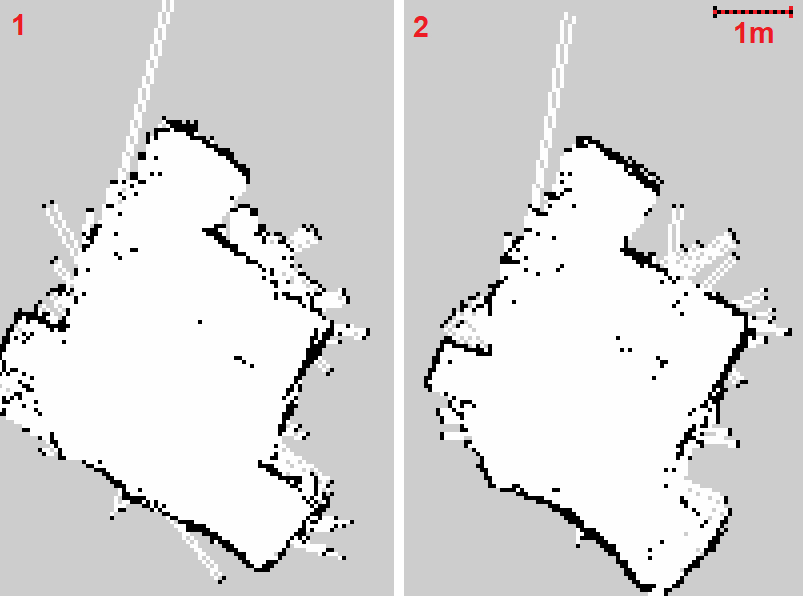
\includegraphics[width=1\linewidth]{rys/saved-map-final-1and2-cropped-upscaled-withscale.png}
	\caption{Mapa pomieszczenia powstała podczas jazdy autonomicznej robota}
    \label{fig:final-scans}
\end{figure}
\chapter{Podsumowanie}
\section{Ocena własna projektu}
>TODO uzupełnić, wyrazić zadowolenie z wyników przeprowadzonych doświadczeń, szczególnie UMBmark który wykazał że projekt podwozia jest dobry

\section{Wnioski}
>TODO uzupełnić


%\bibliographystyle{plalpha}
\bibliographystyle{plabbrv}

\setlength{\bibitemsep}{2pt}
\bibliography{my-bibliography.bib}
\appendix
\chapter{Opis załączonej płyty CD/DVD}
\label{sec:disc-addon}
%>TODO opisać co znajduje się na płycie CD

%na pewno zawrzyj projekt 3d
%do tego dodaj aplikacje pc
%oraz firmware
%moze jakas instrukcje?

\chapterstyle{noNumbered}
\phantomsection
\addcontentsline{toc}{chapter}{Indeks rzeczowy}
\printindex

\end{document}


% 1. Preferowany rozmiar czcionki to 11 lub 12 pkt (mniejsza czcionka może być zastosowana do podpisów rysunków/tabel/równań), interlinia 1.0 lub 1.5.

% 2. Każdy zamieszczony element typu rysunek/tabela/równanie musi mieć swój numer. Rysunki i tabele muszą mieć ten opis.

% 3. Do elementów typu rysunek/tabela/równanie odwołujemy się za pomocą jego numeru, czyli np. "Rysunek 1 przedstawia...". Nie stosujemy sformułowań typu "na rysunku poniże/powyżej".

% 4. Podpis/opis tabeli zamieszczamy nad tabelą, podpis/opis rysunku - pod rysunkiem. Numery równań podajemy w tej samej linii co równanie, po prawej stronie.

% 5. W pracy musi znajdować się bibliografia, a każda pozycja zawarta w bibliografii musi być przynajmniej raz zacytowana. Do cytowania używamy nawiasów klamrowych, w których znajduje się klucz (najczęściej numer) określonej pozycji bibliograficznej. Np. [1] czy też [10].

% 6. Pisząc pracę pamiętamy o ciąg przyczynowo-skutkowym oraz tym, że czytelnik na etapie i-tego rodziału nie wie co przedstawione jest w rozdziale (i+1).

% 7. Każdy akronim użyty w pracy musi zostać zdefiniowany w miejscu jego pierwszego wystąpienia w tekście. Jeśli używanych akronimów jest wiele warto za początku pracy zamieścić ich spis.

% 8. Rysunki zamieszczone w pracy powinny być Państwa autorstwa. Przy każdym rysunku wzięty z literatury należy zamieścić referencję do pozycji bibliograficznej, z której ten rysunek pochodzi.